\chapter{Two-flavor quark-meson model}
\label{chap:lsm2f}

\TODO{main line: 700 (PT) vs 800 (CO) MeV all models. then ``asides'' that push down.}

\TODO{move this to the start?
The linear sigma model is an effective low-energy model of quantum chromodynamics, so accordingly we should take it seriously only in terms of the shifted fields around the stable ground states, and not in terms of the unshifted fields around the unstable equilibrium at the top of the Mexican hat.
}

\TODO{plot BAG PRESSURE as function of $\mu_Q$ and show how it explains the confinement/deconfinement phase transition!}

\TODO{two inconsistencies: (1) match couplings at tree level although using one-loop potential. (2) neglecting bosonic one-loop contribution to effective potential (this is consistent in $N_c\rightarrow \infty$ limit, but inconsistent in terms of number of loops)}

\TODO{Kyllingstad has many sources for showing that pion condensate forms only when $\mu_i > m_\pi / (2)$ (just after figure 1.5). He also has a more applicable phase diagram?}

At low energy, the effective degrees of freedom of quantum chromodynamics are not individual quarks,
but nucleons composed of up and down quarks and the three pions that we saw arose from the spontaneous chiral symmetry breaking pattern \eqref{eq:qcd:symmetry_breaking_pattern}.
The MIT bag model that we discussed in \cref{chap:mit} modeled quark stars by simply confining a free Fermi gas of quarks in baryons with a bag constant $B$.
We will now crank up the difficulty and investigate the \textbf{linear sigma model}, which also takes chiral symmetry breaking and the resulting pions into account by introducing an ``ad--hoc'' $\sigma$ particle.
For example, we will see that the bag pressure that was constant in the MIT bag model now changes throughout the star, describing a transition from deconfined to confined quark matter.
The linear sigma model was originally introduced by \cite{ref:lsm_original} as an effective model for nucleons interacting with pions and scalar mesons.
We will interpret the fermions as quarks instead of nucleons in what is then commonly referred to as a \textbf{quark-meson model}.

The physical justification for this effective model of quantum chromodynamics is best made retrospectively after seeing exactly how it gives rise to chiral symmetry breaking.
We will therefore take the model as granted from the start and justify it as we go along.

\begin{figure}
\centering
\tikzsetnextfilename{potential}
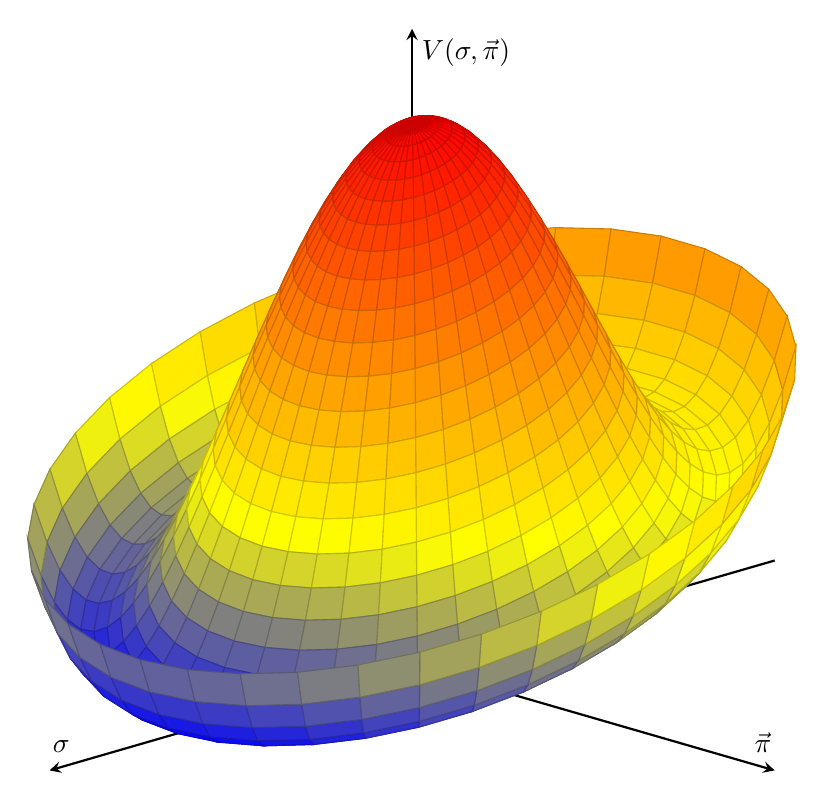
\begin{tikzpicture}
\begin{axis}[
	width = 20cm, height=15cm,
	%title = {Potential},
	xlabel = $\sigma$, ylabel = $\vec\pi$, zlabel = {$V(\sigma,\vec\pi)$},
	xmin=-4.0, xmax=+4.0, ymin=-4.0, ymax=+4.0, zmin=0, zmax=2.2,
	xtick=\empty, ytick=\empty, ztick=\empty,
	axis lines=center,
	axis line style = thick,
	view={135}{25},
	%colormap/blackwhite, mesh/interior colormap name=plasmarev,
]
	\addplot3 [surf, thin, domain=0:3.0, domain y=0:2*pi, samples=30, samples y=40, z buffer=sort] ({x*cos(deg(y))},{x*sin(deg(y))},{-1/2*((x*cos(deg(y)))^2+(x*sin(deg(y)))^2) + 1/24*((x*cos(deg(y)))^2+(x*sin(deg(y)))^2)^2 + 3/2 - 0.15*x*cos(deg(y)) + 0.15*sqrt(6)});
	%\addplot3 [domain=0:2*pi, samples=50, samples y=1] ({sqrt(6)*cos(deg(x))},{sqrt(6)*sin(deg(x))},{0});
\end{axis}
\end{tikzpicture}
\caption{\label{fig:lsm:potential}%
	A two-dimensional realization of the potential \eqref{eq:lsm:potential} looks like a Mexican hat, tilted along the $\sigma$-axis by the explicit symmetry breaking parameter $h$.
	If $h = 0$, the hat is upright with a continuous range of minima around $\sigma^2 + \vec\pi^2 = -6m^2 / \lambda$;
	while if $h \neq 0$, the hat is tilted and has the discrete minimum \eqref{eq:lsm:ground_state_implicit}.
}
\end{figure}

\section{Lagrangian and symmetries}

The Lagrangian density for the linear sigma model coupled to quarks is \cite{ref:jo_lsm_consistent_physical}
\begin{equation}
	\lagr = \bar{q} \Big[ i \slashed\partial + \mu \gamma^0 - g \big( \sigma + i \gamma^5 \vec\tau \cdot \vec\pi \big) \Big] q
	      + \frac12 \Big[ \big( \partial_\mu \sigma \big)^2 + \big( \partial_\mu \vec\pi \big)^2 \Big] - \pot(\sigma,\vec\pi)
\label{eq:lsm:lagrangian}
\end{equation}
with the meson potential
\begin{equation}
	\pot(\sigma, \vec\pi) = \frac{m^2}{2} \big( \sigma^2 + \vec\pi^2 \big) + \frac{\lambda}{4!} \big( \sigma^2 + \vec\pi^2 \big)^2 - h \sigma .
\label{eq:lsm:potential}
\end{equation}
The quark fields behave as in the MIT bag model Lagrangian \eqref{eq:mit:lagrangian} with $N_f=2$ flavor indices $u$ and $d$, $N_c=3$ color indices and four Dirac spinor indices, and are coupled to two chemical potentials $\mu = \diag (\mu_u, \mu_d)$.
However, they are now seemingly massless and coupled to the bosonic $\sigma$ meson and three pions $\vec\pi = [\pi^+, \pi^-, \pi^0]^T$ with a Yukawa coupling $g$ and the Dirac matrices \eqref{eq:tft:pauli_matrices}.
The meson potential features three couplings: $m^2<0$, $\lambda>0$ and $h>0$ \TODO{verify signs from numerical results!}.

Like the quantum chromodynamics Lagrangian \eqref{eq:qcd:lagrangian}, the quark-meson model Lagrangian \eqref{eq:lsm:lagrangian} has the vector $U(1)_V$ and axial $U(1)_A$ symmetry shown in \cref{sec:qcd:symmetry}.
In contrast to the mass-conditional chiral symmetry of the former Lagrangian, however, the latter is \emph{unconditionally} invariant under chiral symmetry $SU(2)_L \times SU(2)_R$ when $h=0$ and $\mu = 0$.
To see this, first rewrite the Yukawa coupling term in terms of left-handed and right-handed chiral fields:
\begin{equation}
\begin{aligned}
	\bar{q} \big[\sigma + i \gamma^5 \vec{\tau} \cdot \vec{\pi}\big] q &= \bar{q} \big[ (P_+ + P_-) \sigma + (P_+ - P_-) i \vec{\tau} \cdot \vec{\pi}\big] q && \; \big( P_\pm = \tfrac{1}{2} (1 \pm \gamma^5) \big) \\
	                                                           %&= \bar{q} \big[ P_+ (\sigma + i \vec{\tau} \cdot \vec{\pi}) + P_- (\sigma - i \vec{\tau} \cdot \vec{\pi}) \big] q && \; \big( \text{distributivity} \big)\\
	                                                           &= \bar{q} \big[ P_+ \phi + P_- \phi^\dagger\big] q && \; \big( \text{define } \phi=\sigma+i\vec{\tau}\cdot\vec{\pi} \big) \\
	                                                           &= \bar{q} \big[ P_+^2 \phi + P_-^2 \phi^\dagger\big] q && \; \big( \text{$P_\pm=P_\pm^2$ lives in spinor-space} \big) \\
	                                                           &= \bar{q} \big[ P_+ \phi P_+ + P_- \phi^\dagger P_-\big] q && \; \big( \text{$\phi$ lives in flavor-space} \big)\\
	                                                           &= \bar{q}_- \phi q_+ + \bar{q}_+ \phi^\dagger q_- && \; \big( \text{$P_\pm q = q_\pm$, $\bar{q} P_\pm = (P_\mp q)^\dagger \gamma^0 = \bar{q}_\mp$} \big).\\
\end{aligned}
\label{eq:lsm:yukawa_symmetry}
\end{equation}
Second, observe that the meson potential \eqref{eq:lsm:potential} with $h=0$ only depends on the flavor-space trace
\begin{equation}
	\tfrac12 \trace\big[\phi^\dagger \phi\big] = \tfrac12 \big( \underbrace{\trace\big[1\big]}_2 \sigma^2 - i^2 \underbrace{\trace\big[\tau_a \tau_b \big]}_{2 \delta_{ab}} \pi_a \pi_b \big) = \sigma^2 + \vec{\pi}^2.
\label{eq:lsm:meson_symmetry}
\end{equation}
Under the $SU(2)_L \times SU(2)_R$ transformation 
\begin{equation}
	q_+ \rightarrow U_+ q_+, \qquad
	q_- \rightarrow U_- q_-
	\qquad \text{and} \qquad
	\phi   \rightarrow U_- \phi U_+^\dagger
\end{equation}
the Yukawa interaction \eqref{eq:lsm:yukawa_symmetry},
the meson potential argument \eqref{eq:lsm:meson_symmetry}
and hence the Lagrangian \eqref{eq:lsm:lagrangian} are invariant.
This proves the claimed unconditional $SU(2)_L \times SU(2)_R$ symmetry when $h=0$ and $\mu=0$.
Since the group $SU(2)_L \times SU(2)_R$ is isomorphic to $O(4)$,
the symmetry can equivalently be understood by considering the meson fields as a four-vector $[\sigma, \vec{\pi}]^T$
and noting that the meson potential \eqref{eq:lsm:potential} is invariant under rotation of this vector in $O(4)$.

What can be the relevance of this unconditional symmetry,
when it was precisely the \emph{breaking} of chiral symmetry that led to the pions of quantum chromodynamics in \cref{sec:qcd:symmetry}?
In vacuum the fermions do not contribute to the grand potential,
and the ground state values $\sigma = \avg{\sigma}$ and $\vec{\pi} = \avg{\vec{\pi}}$ are given by minima of the meson potential $\pot(\avg{\sigma},\avg{\vec{\pi}})$ illustrated in \cref{fig:lsm:potential}.
From equation \eqref{eq:lsm:potential} we see that they are given by
\begin{equation}
	%\vec{\pi} = \avg{\vec{\pi}}
	%\quad \text{and} \quad
	%\sigma = \avg{\sigma}
	%\pdv{\pot}{\sigma}_{(\sigma,\vec\pi)=(\avg{\sigma},\vec{0})} = m^2 \avg{\sigma} + \frac{\lambda}{6} \avg{\sigma}^3 - h = 0.
	\pdv{\pot}{\pi_a} = \avg{\pi_a} \Big[ m^2 + \frac{\lambda}{6} \big(\avg{\sigma}^2 + \avg{\vec{\pi}}^2\big) \Big] = 0
	\quad \text{and} \quad
	\pdv{\pot}{\sigma} = \avg{\sigma} \Big[ m^2 + \frac{\lambda}{6} \big(\avg{\sigma}^2 + \avg{\vec{\pi}}^2\big) \Big] - h = 0.
\label{eq:lsm:ground_state_implicit}
\end{equation}
The qualitative nature of the solutions depend on whether $h$ vanishes.
\begin{itemize}
\item In the \textbf{chiral limit} $h=0$,
      the ground state solutions are a degenerate range of stable minima along the circle $\avg{\sigma}^2+\avg{\vec{\pi}}^2=-6m^2/\lambda$.
      Without any loss of generality, let us pick the one located at $\avg{\sigma} = \sqrt{-6m^2/\lambda}$ and $\avg{\vec{\pi}}=0$.
\item At the \textbf{physical point} $h \neq 0$,
      the ground state is discrete and located at $\avg{\sigma} \neq 0$ and $\avg{\vec{\pi}}=0$ determined implicitly by \eqref{eq:lsm:ground_state_implicit}.
\end{itemize}
Note that $\avg{\vec{\pi}} = 0$ in both cases.
To account for quantum fluctuations $\tilde{\sigma}$ and $\tilde{\vec{\pi}}$ around the ground states, let us write
\begin{equation}
	\sigma = \avg{\sigma} + \tilde{\sigma}
	\qquad \text{and} \qquad
	\vec\pi = \avg{\vec\pi} + \tilde{\vec{\pi}}.
\end{equation}
Up to second order in the quantum fluctuations,
the Lagrangian \eqref{eq:lsm:lagrangian} becomes
\begin{equation}
	\lagr = \sum_{c=1}^{N_c} \bar{q}_c \Big[ i \slashed\partial + \mu \gamma^0 - m_q \Big] q_c
	      + \frac12 \left[ \left( \partial_\mu \tilde{\sigma} \right)^2 + \left( \partial_\mu \tilde{\vec\pi} \right)^2 \right] - \pot(\sigma,\vec\pi) , %\pot(\avg{\sigma}+\tilde{\sigma},\avg{\vec\pi}+\tilde{\vec\pi}) ,
\end{equation}
and the meson potential \eqref{eq:lsm:potential} becomes
\begin{equation}
	\pot(\sigma,\vec\pi) = \pot(\avg{\sigma},\avg{\vec\pi}) + h \tilde{\sigma} + \frac12 m_\sigma^2 \tilde{\sigma}^2 + \frac12 m_\pi^2 \tilde{\pi}^2.
\end{equation}
The quarks $q$, $\sigma$ and $\vec\pi$ fields have acquired the effective masses
\begin{subequations}
\begin{align}
	m_q &= g \avg{\sigma}, \label{eq:lsm:mass_quark} \\
	m_\sigma^2 &= \pdv[2]{\pot}{\sigma}\iffalse_{\substack{\sigma=\avg{\sigma}\\\vec{\pi}=\avg{\vec{\pi}}}}\fi    = m^2 + \frac{\lambda}{2} \avg{\sigma}^2 \equalexplabove{\text{by \eqref{eq:lsm:ground_state_implicit}}} \frac{3h}{\avg{\sigma}} - 2 m^2 , \label{eq:lsm:mass_sigma} \\
	m_\pi^2    &= \pdv[2]{\pot}{\vec{\pi}}\iffalse_{\substack{\sigma=\avg{\sigma}\\\vec{\pi}=\avg{\vec{\pi}}}}\fi = m^2 + \frac{\lambda}{6} \avg{\sigma}^2 \equalexplbelow{\text{by \eqref{eq:lsm:ground_state_implicit}}} \frac{h}{\avg{\sigma}} . \label{eq:lsm:mass_pi}
\end{align}%
\label{eq:lsm:mass_sigmapi}%
\end{subequations}%
The qualitative nature of the pions depends on whether $h$ vanishes.
\begin{itemize}
\item In the \textbf{chiral limit} $h = 0$ the $SU(2) \times SU(2)$ symmetry \eqref{eq:lsm:meson_symmetry} is exact,
      and we saw above that there is a degenerate range of ground states.
      Upon committing to the minimum above, the $O(4)$ rotation symmetry of the original four meson fields $[\sigma,\vec\pi]^T$ are spontaneously broken
      to rotation of only the three pion quantum fluctuations $\tilde{\vec\pi}$ in $O(3)$.
      Accordingly, the pion mass \eqref{eq:lsm:mass_pi} vanishes and so that the three pions are indeed Goldstone bosons associated with spontaneous symmetry breaking.
\item At the \textbf{physical point} $h \neq 0$, the $SU(2) \times SU(2)$ symmetry \eqref{eq:lsm:meson_symmetry} is explicitly broken,
      and we saw above that there is a unique ground state.
      Accordingly, the pion gains a small mass \eqref{eq:lsm:mass_pi}.
\end{itemize}
\label{elaborate on mexican hat analogy, brim, tip/tilt, etc.}
In neither case does the $\sigma$ mass \eqref{eq:lsm:mass_sigma} vanish -- there is no reason for it do so.

The gist of the linear sigma model and its physical justification is this (take a breath):
although the linear sigma model symmetry breaking pattern
\begin{equation}
	SU(2) \times SU(2) \simeq O(4) \qquad \longrightarrow \qquad O(3)
\end{equation}
is \emph{different} from the quantum chromodynamics symmetry breaking pattern \eqref{eq:qcd:symmetry_breaking_pattern} ``under the hood'',
it gives rise to the \emph{same} degrees of freedom (pions) ``on the outside'' and is therefore indistinguishable from it.
This was achieved by the specific Lagrangian \eqref{eq:lsm:lagrangian} with a $\sigma$ particle in addition to the three pions.
The parameter $h \neq 0$ only serves to explicitly break this into an approximate symmetry,
just like the quark masses break the chiral symmetry of quantum chromodynamics.
According to Weinberg's philosophy presented in \cref{sec:qcd:phase_diagram_and_methods},
the quark-meson model is therefore an appropriate effective model of quantum chromodynamics at low energy.


\section{Mass-radius solutions}

\TODO{move afterwards}


\section{Grand potential and equation of state}

\TODO{fix flavor sum indices. make consistent with earlier stuff.}

\TODO{write $\Omega(\avg{\sigma},\vec{\mu})$ in order to keep function declaration general for ``any'' chemical potential combination?}

\TODO{resolve $\avg{\sigma}$ vs $m_q$ variable use}

We now set out to calculate the grand potential \eqref{eq:master_intro:grand_potential}.
With the fermionic quark fields $q$ and bosonic meson fields $\sigma$ and $\vec\pi$
and the coupling of chemical potentials $\mu$ to conserved currents already baked into the Lagrangian \eqref{eq:lsm:lagrangian},
the partition function \eqref{eq:master_intro:partition_function} becomes
\begin{equation}
	Z = \oint_- \pathintdif \bar{q} \oint_- \pathintdif q \oint_+ \pathintdif \sigma \oint_+ \pathintdif \vec\pi \exp \left\{ \int_0^\beta \dif \tau \int_V \dif^3 x \, \lagr_E[\bar{q}, q, \sigma, \vec\pi]  \right\} .
\end{equation}
To calculate it we will use the \emph{mean-field approximation} for the bosonic fields,
replacing them by their yet unknown expectation values $\avg{\sigma}$ and $\avg{\vec\pi}$ in the classical ground state
(all we know is that $\avg{\sigma}=f_\pi$ in vacuum)
and simply ignoring the quantum fluctuations $\tilde{\sigma}$ and $\tilde{\vec\pi}$.
In contrast we will give fermionic fields the full treatment.
In other words, we are treating bosons to tree-level and fermions to one-loop level
-- we will comment more on this seemingly inconsistent approach later.
\TODO{would boson contribution vanish in $T=0$ anyway?}
The precise values of the meson mean fields are determined in retrospect as minima of the grand potential according to
\TODO{say mean field is ``order parameter''. why not parametrize with it? call this gap equation? determine $\avg{\sigma}$ self-consistently}
\begin{equation}
	\pdv{\Omega}{\avg{\sigma}} = \pdv{\Omega}{\avg{\vec\pi}} = 0.
\label{eq:lsm:gap_equation}
\end{equation}
In our treatment we will also neglect pion condensation and \emph{assume} that $\avg{\vec\pi}=0$ \emph{always} vanishes
and only $\avg{\sigma}$ needs to be determined.
This is known to be true at $T=0$ when the isospin chemical potential \eqref{eq:master_intro:chemical_potentials_transformed} does not exceed half the pion mass
-- see for example the study of pion condensation in the quark-meson model by \cite{ref:jo_lsm_consistent,ref:jo_lsm_pion_condensation}.
After inserting the Lagrangian \eqref{eq:lsm:lagrangian} the partition function reads
\begin{equation}
	Z = \prod_{f=1}^{\smash{N_f}} \prod_{c=1}^{\smash{N_c}} \oint_- \!\! \pathintdif \bar{q}_{f,c} \oint_- \!\! \pathintdif q_{f,c} \exp \Bigg\{ \int_0^{\beta} \dif \tau \int_V \dif^3 x \Bigg[ \sum_{f=1}^{\smash{N_f}} \sum_{c=1}^{N_c} \bar{q}_{f,c} \big( i \slashed\partial - m_q + \mu_f \gamma^0 \big) q_{f,c} - \pot(\avg{\sigma},\vec{0}) \Bigg] \Bigg\}.
\end{equation}
The meson potential is independent of the fields and can be pulled out of the integrals,
while the fermionic contribution decouples into a product of identical integrals.
We therefore have
\begin{equation}
\begin{split}
	%\log Z &= -\frac12 \beta V m^2 \avg{\sigma}^2 - \frac{\lambda}{4!} \beta V \avg{\sigma}^4 + \beta V h \avg{\sigma} \\
	       %&+ \sum_{f=1}^{N_f} \sum_{c=1}^{N_c} \log \oint_- \pathintdif \bar{q}_f^c \oint_- \pathintdif q_f^c \exp \left\{ \int_0^\beta \dif \tau \int_V \dif^3 x \, \bar{q}_f^c (i \slashed\partial + \mu_f \gamma^0 - m_q) q_f^c \right\} .
	\log Z = -\pot(\avg{\sigma},\vec{0}) + \sum_{f=1}^{N_f} \sum_{c=1}^{N_c} \log \oint_- \!\! \pathintdif \bar{q}_{f,c} \oint_- \!\! \pathintdif q_{f,c} \exp \bigg\{ \! \int_0^\beta \! \dif \tau \int_V \! \dif^3 x \, \bar{q}_{f,c} \big(i \slashed\partial + \mu_f \gamma^0 - m_q\big) q_{f,c} \! \bigg\} .
\end{split}
\end{equation}
We have already calculated the path integral in the last term
from equation \eqref{eq:tft:dirac_partition_function_first} to equation \eqref{eq:tft:dirac_partition_function}.
Here we get an additional factor $\sum_{c=1}^{N_c} = N_c$ from the color sum because the summand is independent of $c$,
while the flavor sum $\sum_{f=1}^{\smash{N_f}}$ yields $N_f$ terms that differ only by the unique chemical potentials $\mu_f$ associated with each quark flavor. 
Thus, the grand potential \eqref{eq:master_intro:grand_potential} is
\begin{equation}
\begin{split}
	%\log Z &= -\frac12 \beta V m^2 \avg{\sigma}^2 - \frac{\lambda}{4!} \beta V \avg{\sigma}^4 + \beta V h \avg{\sigma} \\
	       %&+ 2 V N_c \sum_{f=1}^{N_f} \int \frac{\dif^3 p}{(2 \pi)^3} \left\{ \beta E(\vec{p}) + \log \left[ e^{-\beta (E(\vec{p}) - \mu_f)}+1 \right] + \log \left[ e^{-\beta (E(\vec{p}) + \mu_f)} + 1\right] \right\} ,
	\Omega = \pot(\avg{\sigma},\vec{0}) - \frac{2 N_c}{\beta} \sum_{f=1}^{N_f} \int \frac{\dif^3 p}{(2 \pi)^3} \left\{ \beta E(\vec{p}) + \log \left[ e^{-\beta (E(\vec{p}) - \mu_f)}+1 \right] + \log \left[ e^{-\beta (E(\vec{p}) + \mu_f)} + 1\right] \right\} ,
\end{split}
\label{eq:lsm:potential_divergent_logz0}
\end{equation}
with the dispersion relation $E(\vec{p}) = \sqrt{\smash[b]{p^2 + m_q^2}}$.

% equivalent remark is made in Folkestad/Andersen 2019 "Thermodynamics and phase diagram of Polykaov-loop extended chiral models"
Note that the fermionic contribution to the grand potential \eqref{eq:lsm:potential_divergent_logz0} is of order $\bigo(N_c)$,
while any bosonic contribution is only of order $\bigo(1)$.
This means that our approach of excluding bosonic fluctuations that sounds very \emph{inconsistent} in one regard
would be \emph{exact} in the limit $N_c \rightarrow \infty$
and can therefore be viewed as \emph{consistent} in the so-called large-$N_c$ approximation.
Although $N_c = 3$ in nature and it may sound like we are not making a great case for ourselves,
this is in fact a widely used \TODO{?} approximation scheme of quantum chromodynamics
and the most common treatment found in the literature.
\TODO{comment on another inconsistency elsewhere: match parameters at tree-level, but later with one-loop effects. but this is another inconsistency, where bosonic fluctuations are still excluded?}

Like before we work in the zero-temperature approximation $T=0$ and choose positive chemical potentials so the anti-particle contribution from the last term in curly brackets vanishes.
The middle term in curly brackets was calculated in the zero-temperature pressure $P=-\Omega$ in \eqref{eq:nstars:pressure_zeroT}.
This time we will also include and renormalize the infinite vacuum contribution from the first term in curly brackets.
Reinstating the Fermi momenta $p_f = \sqrt{\smash[b]{\mu_f^2-m_f^2}}$, we obtain
\begin{equation}
	\Omega = -N_c N_f \Omega_0 - \smashoperator{\sum_{\vphantom{\big|} f=\{u,d,s\}}} \frac{N_c}{24 \pi^2} \left[ \left( 2 \mu_f^2 - 5 m_f^2 \right) \mu_f \sqrt{\mu_f^2 - m_f^2} + 3 m_f^4 \asinh \left( \sqrt{\frac{\mu_{\smash{f}}^2}{m_f^2}-1} \right) \right]
\end{equation}
with the vacuum contribution
\begin{equation}
	\Omega_0 = -2 \int \frac{\dif^3 p}{(2 \pi)^3} \sqrt{p^2 + m_q^2}.
\label{eq:lsm:vacuum_contribution_3dim}
\end{equation}
To renormalize it we use dimensional regularization in the minimal subtraction scheme.
In $d = 3 - 2 \epsilon$ spatial dimensions, the vacuum contribution is
\begin{equation}
\begin{split}
	\Omega_0 &= -2 \Lambda^{3-d} \int \frac{\dif^d p}{(2 \pi)^d} \sqrt{p^2 + m_q^2} \\
	         &= -2 \Lambda^{3-d} \frac{2 \pi^{d/2}}{\Gamma(d/2)} \int_0^\infty \frac{\dif p \, p^{d-1}}{(2 \pi)^d} \sqrt{p^2 + m_q^2} .
\end{split}
\label{eq:lsm:vacuum_contribution_ddim}
\end{equation}
%\TODO{what happens to the dimensions of the potential $V$ (as consequence of requiring $\log Z$ to be dimensionless)? $V \rightarrow V \lambda^{-2\epsilon}$?}
We have also multiplied the integral by $\Lambda^{3-d} = \Lambda^{2\epsilon}$ where $\Lambda$ is some number with $\unit{\Lambda} = \unit{p}$,
so that $\unit{\lambda^{3-d} \dif^d p} = \unit{\dif^3 p}$ and $\Omega$ is well-defined with correct \emph{dimension} in all \emph{dimensions}.
There is nothing that forbids us from doing so,
as the regulator still accomplishes its only job of reducing the new integral \eqref{eq:lsm:vacuum_contribution_ddim} to the old integral \eqref{eq:lsm:vacuum_contribution_3dim} when we send $\epsilon \rightarrow 0$.
The momentum integral can be written as an analytical continuation of the \emph{Beta function} \cite{ref:beta_function}
\begin{equation}
	B(x,y) = \int_0^\infty \dif t \, \frac{t^{x-1}}{(1+t)^{x+y}} = \frac{\Gamma(x) \Gamma(y)}{\Gamma(x+y)}
\end{equation}
if we substitute $t = p^2/m_q^2$ with $\dif t = 2 p \dif p / m_q^2$.
We then find
\begin{equation}
\begin{split}
	\Omega_0 &= -\Lambda^{3-d} m_q^{d+1} \frac{2 (4 \pi)^{-d/2}}{\Gamma\big(\frac{d}{2}\big)} \int_0^\infty \dif t \, \frac{t^{d/2-1}}{(1+t)^{-1/2}} \\
	         &= -\Lambda^{3-d} m_q^{d+1} \frac{2 (4 \pi)^{-d/2}}{\Gamma\big(\frac{d}{2}\big)} \frac{\Gamma\big(\frac{d}{2}\big) \Gamma\big( \textstyle{-\frac{d+1}{2}} \big)}{\Gamma\big( \textstyle{-\frac{1}{2}} \big)} .
\end{split}
\end{equation}
We now cancel the two factors $\Gamma(d/2)$ and replace $\Gamma(-1/2) = -2\sqrt{\pi}$.
Then we insert $d = 3 - 2 \epsilon$ back and use the property $\Gamma(z) = \Gamma(z+1) / z$ twice to transport the argument of the Gamma function infinitesimally close to its pole at $0$,
where we use its asymptotic expansion $\Gamma(\epsilon) = 1/\epsilon + \gamma + \bigo(\epsilon)$ upon arrival.
Expanding everything to zeroth order in $\epsilon$ then yields
\begin{equation}
	\Omega_0 =       \frac{m_q^4}{8 \pi^2} \left( 4 \pi \frac{\Lambda^2}{m_q^2} \right)^\epsilon \Gamma(-2 + \epsilon)
	         \taylor \frac{m_q^4}{16 \pi^2} \left( \frac{1}{\epsilon} + \log \frac{\Lambda^2}{m_q^2} + \frac32 - \gamma + \log 4 \pi \right) .
\label{eq:lsm:vacuum_contribution_final}
\end{equation}
In hindsight, we now see that we could get rid of the terms $-\gamma + \log 4 \pi$ if we had rather used the modified minimal subtraction scheme, where one rescales $\Lambda^2 \rightarrow \Lambda^2 e^\gamma / 4 \pi$.
With the vacuum contribution \eqref{eq:lsm:vacuum_contribution_final} in this renormalization scheme, the full logarithm \eqref{eq:lsm:potential_divergent_logz0} becomes
\begin{equation}
\begin{split}
	\Omega &= \pot(\avg{\sigma},\vec{0}) + N_c N_f \frac{m_q^4}{16 \pi^2} \left[ \frac{1}{\epsilon} + \frac{3}{2} + \log\left(\frac{{\Lambda}^2}{m_q^2}\right) \right] \\
	       &- \smashoperator{\sum_{\vphantom{\big|} f=\{u,d\}}} \frac{N_c}{24 \pi^2} \left[ \left( 2 \mu_f^2 - 5 m_f^2 \right) \mu_f \sqrt{\mu_f^2 - m_f^2} + 3 m_f^4 \asinh \left( \sqrt{\frac{\mu_{\smash{f}}^2}{m_f^2}-1} \right) \right]
\end{split}
\end{equation}
This investigation has revealed that the term $N_c N_f m_q^4 / 16 \pi^2 \epsilon$ is responsible for the vacuum divergence.
Recalling that $m_q=g \avg{\sigma}$,
we also see that the divergence can be removed by the term $\lambda \avg{\sigma}^4 / 24$ in the meson potential $\pot(\avg{\sigma},\vec{0})$
if we shift the quartic coupling
\begin{equation}
	\lambda \rightarrow \lambda + \delta\lambda
	\qquad \text{with the counterterm} \qquad
	\delta\lambda = -N_c N_f \frac{3 g^4}{2 \pi^2 \epsilon} .
\end{equation}
Adding free electrons to the mix, the finite and renormalized grand potential is finally
\TODO{fix $m_f$ vs $m_q$}
\begin{equation}
\begin{split}
	\Omega(\avg{\sigma},\mu_u,\mu_d,\mu_e) &= \pot(\avg{\sigma},\vec{0}) + N_c N_f \frac{m_q^4}{16 \pi^2} \left[ \frac{3}{2} + \log\left(\frac{{\Lambda}^2}{m_q^2}\right) \right] \\
	                                       %&- \frac{N_c}{24 \pi^2} \sum_{f=\{u,d\}} \left[ \left( 2 \mu_f^2 - 5 m_q^2 \right) \mu_f \sqrt{\mu_f^2 - m_q^2} + 3 m_q^4 \asinh \left( \sqrt{\frac{\mu_{\smash{f}}^2}{m_q^2}-1} \right) \right] \\
	                                       %&- \frac{  1}{24 \pi^2} \left[ \left( 2 \mu_e^2 - 5 m_e^2 \right) \mu_e \sqrt{\mu_e^2 - m_e^2} + 3 m_e^4 \asinh \left( \sqrt{\frac{\mu_e^2}{m_e^2}-1} \right) \right] .
	                                       &-\smashoperator{\sum_{\vphantom{\big|} f=\{u,d\}}} \frac{N_c}{24 \pi^2} \left[ \left( 2 \mu_f^2 - 5 m_f^2 \right) \mu_f \sqrt{\mu_f^2 - m_f^2} + 3 m_f^4 \asinh \left( \sqrt{\frac{\mu_{\smash{f}}^2}{m_f^2}-1} \right) \right] \\
	                                       &-\phantom{\sum} \, \frac{1}{24 \pi^2} \left[ \left( 2 \mu_e^2 - 5 m_e^2 \right) \mu_e \sqrt{\mu_e^2 - m_e^2} \, \, + \, 3 m_e^4 \asinh \left( \sqrt{\frac{\mu_{\smash{e}}^2}{m_e^2}-1} \right) \right].
\end{split}
\label{eq:lsm:grand_potential}
\end{equation}

The particle densities are the same as in the MIT bag model:
\begin{subequations}
\begin{align}
	n_u &= -\pdv{\Omega}{\mu_u} = \frac{N_c}{3 \pi^2} \Big( \mu_u^2 - m_q^2 \Big)^{\frac32}, \\
	n_d &= -\pdv{\Omega}{\mu_d} = \frac{N_c}{3 \pi^2} \Big( \mu_d^2 - m_q^2 \Big)^{\frac32}, \\
	n_e &= -\pdv{\Omega}{\mu_e} = \frac{  1}{3 \pi^2} \Big( \mu_e^2 - m_e^2 \Big)^{\frac32}.
\end{align}%
\label{eq:lsm:particle_densities}%
\end{subequations}%
The pressure \eqref{eq:master_intro:pressure} and energy density \eqref{eq:master_intro:energy_density} follow straightforwardly from the grand potential \eqref{eq:lsm:grand_potential} and particle densities \eqref{eq:lsm:particle_densities}.

\subsection{Parameter fitting}

\begin{table}
\centering
\begin{tabular}{ l r r }
	\toprule
	Variable & Model value                             & Experimental value \\
	\midrule
	$\avg{\sigma}=f_\pi$ & $\textbf{\SI{93}{\mega\electronvolt}}$  & \SI{92}{}-\SI{93}{\mega\electronvolt} \\
	%\midrule
	$m_u=m_d$            & $\textbf{\SI{300}{\mega\electronvolt}}$ & \approx \, \SI{300}{\mega\electronvolt} \\
	%\midrule
	$m_\sigma$           & $\textbf{\{700,800\}\,\si{\mega\electronvolt}}$ & \SI{400}{}-\SI{700}{\mega\electronvolt}          \\
	$m_\pi$              & $\textbf{\SI{138}{\mega\electronvolt}}$ & \SI{138}{\mega\electronvolt}                     \\
	\\
	\bottomrule
\end{tabular}
\hfill
\begin{tabular}{ l r }
	\toprule
	Parameter   & Model value                           \\
	\midrule
	$g$         & $\SI{3.23}{}$                         \\
	$\lambda$   & $-\{163.4,215.4\}$                        \\
	$m^2$       & $-(\{465.2,539.8\} \, \si{\mega\electronvolt})^2$ \\
	$h$         & $(\SI{121.0}{\mega\electronvolt})^3$  \\
	$\Lambda$   & $\SI{182.0}{\mega\electronvolt}$ \\
	\bottomrule
\end{tabular}
\caption{\label{tab:lsm2f:parameters}%
Parameter fit for the two-flavor linear sigma model in vacuum compared to experimental values from \cite{ref:pdg_review_2021}.
The \textbf{bold values} in the left table are used as input to determine the parameters \eqref{eq:lsm:parameters} and \eqref{eq:lsm:potential_vacuum_minimum}.
Two different values are used for $m_\sigma$, generating two different values of both $\lambda$ and $m^2$, while the remaining parameters remain unchanged.
}
\end{table}

To determine the four paremeters $g$, $m^2$, $\lambda$ and $h$ in the Lagrangian \eqref{eq:lsm:lagrangian},
we use measured values of the mean field $\avg{\sigma}$ and masses $m_\sigma$, $m_\pi$ and $m_q$ in vacuum.
Inverting equations \eqref{eq:lsm:ground_state_implicit}, \eqref{eq:lsm:mass_sigmapi} and \eqref{eq:lsm:mass_quark}, we then find the parameters
\begin{equation}
	g       = \frac{m_q}{f_\pi}, \quad % &\qquad& \text{(by \eqref{eq:lsm:mass_quark})} , \\
	h       = m_\pi^2 f_\pi, \quad % &\qquad& \text{(by \eqref{eq:lsm:mass_pi})} , \\
	m^2     = \frac{3m_\pi^2 - m_\sigma^2}{2} \quad \text{and} \quad % &\qquad& \text{(by \eqref{eq:lsm:mass_sigma})} , \\
	\lambda = \frac{3 m_\sigma^2 - 3 m_\pi^2}{f_\pi^2} .    % &\qquad& \text{(by \eqref{eq:lsm:ground_state_implicit})} .
\label{eq:lsm:parameters}
\end{equation}
According to \cite{ref:pdg_review_2021}, in vacuum the mean field $\avg{\sigma} = f_\pi = \SI{93}{\mega\electronvolt}$ is the pion decay constant,
$m_\pi = \SI{138}{\mega\electronvolt}$ is the average mass of the three pions
and the up and down quarks have almost equal masses $m_u \approx m_d \approx \SI{300}{\mega\electronvolt}$.
All of these quantities have low uncertainty.

\begin{figure}
\centering
\tikzsetnextfilename{2-flavor-potential-vacuum}
\begin{tikzpicture}
\begin{axis}[
	width = 15cm, height = 7cm,
	xmin=-500, xmax=+500, xtick distance = 100, minor x tick num=9,
	ymin=-11, ymax=+6, ytick distance=5, minor y tick num=4,
	xlabel = {$\Delta \, / \, \si{\mega\electronvolt}$}, ylabel = {$\Omega \, / \, f_\pi^4$},
	legend style = {at={(0.5,1.03)}, anchor=south}, legend columns=4,
	cycle list/YlOrRd-6,
]
\pgfplotsset{cycle list shift=+2} % skip weakest line
\addplot+ [] table [x=Deltax, y=Omega] {../code/data/LSM2F/potential_vacuum_sigma500.dat}; \addlegendentry{$m_\sigma = \SI{500}{\mega\electronvolt}$};
%\addplot+ [] table [x=Deltax, y=Omega] {../code/data/LSM2F/potential_vacuum_sigma550.dat}; \addlegendentry{$m_\sigma = \SI{550}{\mega\electronvolt}$};
\addplot+ [] table [x=Deltax, y=Omega] {../code/data/LSM2F/potential_vacuum_sigma600.dat}; \addlegendentry{$m_\sigma = \SI{600}{\mega\electronvolt}$};
%\addplot+ [] table [x=Deltax, y=Omega] {../code/data/LSM2F/potential_vacuum_sigma650.dat}; \addlegendentry{$m_\sigma = \SI{650}{\mega\electronvolt}$};
\addplot+ [] table [x=Deltax, y=Omega] {../code/data/LSM2F/potential_vacuum_sigma700.dat}; \addlegendentry{$m_\sigma = \SI{700}{\mega\electronvolt}$};
%\addplot+ [] table [x=Deltax, y=Omega] {../code/data/LSM2F/potential_vacuum_sigma750.dat}; \addlegendentry{$m_\sigma = \SI{750}{\mega\electronvolt}$};
\addplot+ [] table [x=Deltax, y=Omega] {../code/data/LSM2F/potential_vacuum_sigma800.dat}; \addlegendentry{$m_\sigma = \SI{800}{\mega\electronvolt}$};
%\addplot+ [] table [x=Deltax, y=Omega] {../code/data/LSM2F/potential_vacuum_sigma850.dat}; \addlegendentry{$m_\sigma = \SI{850}{\mega\electronvolt}$};
\end{axis}
\end{tikzpicture}
\caption{\label{fig:lsm:potential_sigma_mass}\TODO{caption}
Two-flavor vacuum potential with
$\mu_u = \mu_d = \mu_e = 0$}
\end{figure}

On the other hand, the mass $m_\sigma$ is very uncertain and hard to choose.
Even in 2002, according to the $\sigma$ meson status update \cite{ref:sigma_meson_status},
it was only known to lie in the huge uncertainty range $\SI{400}{\mega\electronvolt} < m_\sigma < \SI{1200}{\mega\electronvolt}$.
Today \cite{ref:pdg_review_2021} places it in the tighter range $\SI{400}{\mega\electronvolt} < m_\sigma < \SI{550}{\mega\electronvolt}$.
Ideally we would like to use a value within this range, but there are several problems.
First, the vacuum potential $\pot(\avg{\sigma},\vec{0})$ plotted in \cref{fig:lsm:potential_sigma_mass} does not have a minimum and is therefore useless for $m_\sigma \lesssim \SI{500}{\mega\electronvolt}$.
In \cref{chap:lsm3f} we will see that the same happens in the three-flavor case, only then for even greater masses $m_\sigma \lesssim \SI{700}{\mega\electronvolt}$.
Since we would like to compare the results obtained with two and three flavors,
we decide to mainly operate with two common values $m_\sigma = \{700,800\} \, \si{\mega\electronvolt}$.
\TODO{present $m_\sigma=600$ results too unless too messy}
The two different values will illustrate qualitatively different behaviors of the chiral phase transition.
This is the best we can do and must be regarded as a shortcoming of our model.

The $\sigma$ meson is controversial and was introduced in an unsatisfying and ad-hoc manner anyway,
in a sense only to make way for the pions that are known low-energy effective degrees of freedom of quantum chromodynamics.
Perhaps cynically, we therefore argue that if \emph{someone} must be treated badly for the model to even function,
the $\sigma$ meson brings with it the least severe physical consequences and is the most deserving candidate.

Note that the renormalization procedure also introduced an unknown parameter $\Lambda$.
To determine it, we require that the minimum of the grand potential \eqref{eq:lsm:grand_potential}
remains at the minimum $\avg{\sigma} = f_\pi$ of the vacuum potential $\pot(\avg{\sigma},\vec{0})$.
Since $\pdv{\pot}/{\avg{\sigma}} = 0$ at $\avg{\sigma}=f_\pi$ already by assumption, we only need
\begin{equation}
	\pdv{\Omega}{\avg{\sigma}}_{\avg{\sigma}=f_\pi} =
	\pdv*{\Bigg[ N_c N_f \frac{m_q^4}{16 \pi^2} \bigg( \frac32 + \log \frac{\Lambda^2}{m_q^2} \bigg) \Bigg] }{\avg{\sigma}} = 0,
	\qquad \text{yielding} \qquad
	\Lambda = \frac{g f_\pi}{\sqrt{e}}.
\label{eq:lsm:potential_vacuum_minimum}
\end{equation}

\Cref{tab:lsm2f:parameters} summarizes the chosen input values for $\avg{\sigma}=f_\pi$, $m_\pi$, $m_\sigma$ and $m_q$ and the corresponding output parameters $m^2$, $\lambda$, $g$, $h$ and $\Lambda$.

Also note that we have treated bosons and fit the parameters of the model using the \emph{tree level} masses \eqref{eq:lsm:mass_sigmapi},
but handled fermions to one loop. 
This is also inconsistent, as the tree-level masses would really receive radiative loop corrections.
We will later investigate the effects of fitting the parameters consistently at one loop level.

\subsection{Equation of state}

\begin{figure}
\centering
\tikzsetnextfilename{grand-potential-noisospin}
\begin{tikzpicture}
\begin{groupplot}[
	group style={group size={2 by 1}, vertical sep=2.0cm, horizontal sep=0.05cm},
	view={170}{25},
	width=0.55\textwidth, height=8cm,
	xlabel = {$m_q \, / \, \si{\mega\electronvolt}$},
	colormap/OrRd, point meta min=0, point meta max=600,
	3d box=complete,
	unbounded coords=jump, % skip at nan (i.e. the phase transition)
	extra tick style={grid=major, grid style={dashed}},
	title style={text width={5cm}},
	xlabel style={sloped}, 
	ylabel style={sloped, xshift=-0.5cm}, yticklabel style={anchor=east},
	zticklabels={,,},
	title style={sloped like x axis},
%
	zmin=-40, zmax=+10,
	xmin=-525, xmax=+525,
	restrict x to domain=-550:+550,
	restrict z to domain=-50:+30,
	xtick distance=150, %minor x tick num=1,
	ytick distance=100, %minor y tick num=3,
]
\nextgroupplot[
	ylabel = {$\mu \, / \, \si{\mega\electronvolt}$},
	%zlabel = {$\Omega(m_q, \mu) \, / \, (\SI{100}{\mega\electronvolt})^4$},
	zlabel = {$\Omega(m_q, \mu)$},
	title = {\subcaption{\label{fig:lsm:grand-potential-noisospin-sigma700}$m_\sigma=\SI{700}{\mega\electronvolt}$}},
];
\addplot3 [surf, very thin, mesh/ordering=x varies, point meta={abs(\thisrow{Delta})}] table [x=Delta, y=mu, z=Omega] {../code/data/LSM2F/potential_noisospin_sigma_700.dat};
\addplot3 [blue, x filter/.expression={\thisrow{Delta0} < 150 ? x : nan}] table [x=Delta0, y=mu0, z=Omega0]     {../code/data/LSM2F/potential_noisospin_sigma_700.dat}; % plot line of minima
\addplot3 [blue, x filter/.expression={\thisrow{Delta0} > 150 ? x : nan}] table [x=Delta0, y=mu0, z=Omega0]     {../code/data/LSM2F/potential_noisospin_sigma_700.dat}; % plot line of minima
\addplot3 [gray, x filter/.expression={\thisrow{Delta0} < 150 ? x : nan}] table [x=Delta0, y=mu0, z expr={-40}] {../code/data/LSM2F/potential_noisospin_sigma_700.dat}; % plot its "shadow" in bottom plane
\addplot3 [gray, x filter/.expression={\thisrow{Delta0} > 150 ? x : nan}] table [x=Delta0, y=mu0, z expr={-40}] {../code/data/LSM2F/potential_noisospin_sigma_700.dat}; % plot its "shadow" in bottom plane
\nextgroupplot[
	yticklabels={,,},
	zticklabels={,,},
	title = {\subcaption{\label{fig:lsm:grand-potential-noisospin-sigma800}$m_\sigma=\SI{800}{\mega\electronvolt}$}},
];
\addplot3 [surf, very thin, mesh/ordering=x varies, point meta={abs(\thisrow{Delta})}] table [x=Delta, y=mu, z=Omega] {../code/data/LSM2F/potential_noisospin_sigma_800.dat};
\addplot3 [blue] table [x=Delta0, y=mu0, z=Omega0]     {../code/data/LSM2F/potential_noisospin_sigma_800.dat}; % plot line of minima
\addplot3 [gray] table [x=Delta0, y=mu0, z expr={-40}] {../code/data/LSM2F/potential_noisospin_sigma_800.dat}; % plot its "shadow" in bottom plane
\end{groupplot}
\end{tikzpicture}
\caption{\label{fig:lsm:grand-potential-noisospin}%
	The grand potential \eqref{eq:lsm:grand_potential} with zero isospin, or $\mu_u = \mu_d = \mu$ and $\mu_e=0$, for $m_\sigma=\{700,800\} \, \si{\mega\electronvolt}$.
	The \textcolor{blue}{blue line} and its \textcolor{gray}{gray projection} show minima of $m_q = g \avg{\sigma}$ determined by $\pdv{\Omega}/{\avg{\sigma}} = 0$.
}
\end{figure}

Before finding the general charge neutral equation of state,
it is easier and instructive to solve the special problem with imposed zero isospin $\mu_I=0$, or $\mu_u=\mu_d=\mu$.
This will give us some intuition for the shape of the grand potential in the general case.
Then the chemical equilibrium constraint \eqref{eq:lsm:chemical_equilibrium} says $\mu_e=0$,
so electrons are absent and only the two first lines in the grand potential \eqref{eq:lsm:grand_potential} contribute.
The grand potential $\Omega(\avg{\sigma},\mu)$ is now a function of two variables that is easy to visualize, as done in \cref{fig:lsm:grand-potential-noisospin}.
We see that:
\begin{itemize}
\item For $\mu < \SI{300}{\mega\electronvolt} = m_q(f_\pi)$ the grand potential is independent of $\mu$,
      and we are in vacuum where only the first line of the grand potential \eqref{eq:lsm:grand_potential} contributes.
      By construction, the minimum lies at $\avg{\sigma} = f_\pi = \SI{93}{\mega\electronvolt}$.
      The feature that a \emph{range} of chemical potentials characterizes the vacuum is sometimes called the \emph{Silver Blaze property}.
\item For $\SI{300}{\mega\electronvolt} < \mu \lesssim \SI{400}{\mega\electronvolt}$,
      the quarks in the second line of the grand potential \eqref{eq:lsm:grand_potential} begins to contribute as we leave the vacuum state.
      For $m_\sigma = \SI{700}{\mega\electronvolt}$ the minimum jumps \emph{discontinuously}, corresponding to a \emph{first-order phase transition}.
      On the other hand, for $m_\sigma = \SI{800}{\mega\electronvolt}$ it moves quickly but still \emph{continuously}, and there is \emph{no phase transition}
      -- this behavior is often referred to as a \emph{crossover}.
\item For $\mu \gtrsim \SI{400}{\mega\electronvolt}$ the minimum approaches the ultra-relativistic limit $m_q \rightarrow 0$ asymptotically, but never quite reaches it.
\end{itemize}

Our objective, however, is to determine the equation of state $\epsilon(P)$ in the general case,
where the chemical potentials are constrained by the conditions of charge neutrality \eqref{eq:lsm:charge_neutrality} and $\beta$-equilibrium \eqref{eq:lsm:chemical_equilibrium} into account.
This means that we must not only solve the gap equation \TODO{I haven't called it this yet} \eqref{eq:lsm:gap_equation},
but the \emph{system} of two equations
\begin{subequations}
\begin{align}
	0 &= \pdv{\Omega}{\avg{\sigma}} , \label{eq:lsm:minsys_min} \\
	%0 &= +\frac23 n_u - \frac13 n_d - n_e , \label{eq:lsm:minsys_charge} \\
	0 &= 2 \Big[\mu_u^2-m_q^2\Big]^\frac32 - \Big[(\mu_u+\mu_e)^2-m_q^2\Big]^\frac32 - \Big[\mu_e^2-m_e^2\Big]^\frac32 \label{eq:lsm:minsys_charge}.
\end{align}%
\label{eq:lsm:minsys}%
\end{subequations}%
for a given value of one variable -- say $\avg{\sigma} = m_q/g$.
The solution yields $\mu_u$ and $\mu_e$, and the remaining chemical potential $\mu_d$ can then be calculated from the equilibrium constraint \eqref{eq:lsm:chemical_equilibrium}.
Parametrizing multiple solutions in this manner, it is straightforward to calculate the densities \eqref{eq:lsm:particle_densities}, pressure \eqref{eq:master_intro:pressure} and energy density \eqref{eq:master_intro:energy_density},
and hence the equation of state $\epsilon(P)$.
The details of the numerical implementation can be found in \cref{sec:num:qstars2f} \TODO{write it}.

\begin{figure}
\centering
\tikzsetnextfilename{2-flavor-eos}
\begin{tikzpicture}
\tikzset{declare function={
	muu(\muQ)=2/(1+2^(1/3))*\muQ;
	mud(\muQ)=2/(1+2^(-1/3))*\muQ;
	mue(\muQ)=2*(2^(1/3)-1)/(2^(1/3)+1)*\muQ;
	nq(\mu)=3/(3*pi^2)*(\mu)^3;
	ne(\mu)=1/(3*pi^2)*(\mu)^3;
	nconv=1.29619e-7;
}};
\begin{groupplot}[
	group style={group size={1 by 3}, vertical sep=2.0cm},
	width=13cm, height=7cm,
	extra tick style={grid=major, grid style={dashed}},
	minor tick num=9,
]
\nextgroupplot[
	xlabel={$\mu_Q \, / \, \si{\mega\electronvolt}$},
	%xmin=0, xmax=600, ymax=500, xtick distance=100, ytick distance=100, minor x tick num=9,
	xmin=0, xmax=600, xtick distance=100, minor x tick num=9,
	ymin=-20, ymax=500, ytick distance=100, 
	%ymax=600, 
	title={\subcaption{\label{fig:lsm:2-flavor-eos-parametrization}Parametrization of solutions }},
	legend cell align=right, legend pos=north west, reverse legend,
];
\addplot+ [orange,    densely dashed, semithick, opacity=0.4, forget plot, domain=0:600] {0};
\addplot+ [red,       densely dashed, semithick, opacity=0.4, forget plot, domain=0:600] {muu(x)};
\addplot+ [darkgreen, densely dashed, semithick, opacity=0.4, forget plot, domain=0:600] {mud(x)};
\addplot+ [blue,      densely dashed, semithick, opacity=0.4, forget plot, domain=0:600] {mue(x)};
\addplot+ [blue,      solid, opacity=0.7             ] table [x expr={(\thisrow{muu}+\thisrow{mud})/2}, y=mue]    {../code/data/LSM2F/eos_sigma_600.dat}; \addlegendentry{$\mu_e \, / \, \si{\mega\electronvolt}$};
\addplot+ [blue,      solid, opacity=0.7, forget plot] table [x expr={(\thisrow{muu}+\thisrow{mud})/2}, y=mue]    {../code/data/LSM2F/eos_sigma_700.dat};
\addplot+ [blue,      solid, opacity=0.7, forget plot] table [x expr={(\thisrow{muu}+\thisrow{mud})/2}, y=mue]    {../code/data/LSM2F/eos_sigma_800.dat};
\addplot+ [darkgreen, solid, opacity=0.7             ] table [x expr={(\thisrow{muu}+\thisrow{mud})/2}, y=mud]    {../code/data/LSM2F/eos_sigma_600.dat}; \addlegendentry{$\mu_d \, / \, \si{\mega\electronvolt}$};
\addplot+ [darkgreen, solid, opacity=0.7, forget plot] table [x expr={(\thisrow{muu}+\thisrow{mud})/2}, y=mud]    {../code/data/LSM2F/eos_sigma_700.dat};
\addplot+ [darkgreen, solid, opacity=0.7, forget plot] table [x expr={(\thisrow{muu}+\thisrow{mud})/2}, y=mud]    {../code/data/LSM2F/eos_sigma_800.dat};
\addplot+ [red,       solid, opacity=0.7             ] table [x expr={(\thisrow{muu}+\thisrow{mud})/2}, y=muu]    {../code/data/LSM2F/eos_sigma_600.dat}; \addlegendentry{$\mu_u \, / \, \si{\mega\electronvolt}$};
\addplot+ [red,       solid, opacity=0.7, forget plot] table [x expr={(\thisrow{muu}+\thisrow{mud})/2}, y=muu]    {../code/data/LSM2F/eos_sigma_700.dat};
\addplot+ [red,       solid, opacity=0.7, forget plot] table [x expr={(\thisrow{muu}+\thisrow{mud})/2}, y=muu]    {../code/data/LSM2F/eos_sigma_800.dat};
\addplot+ [orange,    solid, opacity=0.7             ] table [x expr={(\thisrow{muu}+\thisrow{mud})/2}, y=mu] {../code/data/LSM2F/eos_sigma_600.dat}; \addlegendentry{$\Delta \, / \, \si{\mega\electronvolt}$};
\addplot+ [orange,    solid, opacity=0.7, forget plot] table [x expr={(\thisrow{muu}+\thisrow{mud})/2}, y=mu] {../code/data/LSM2F/eos_sigma_700.dat};
\addplot+ [orange,    solid, opacity=0.7, forget plot] table [x expr={(\thisrow{muu}+\thisrow{mud})/2}, y=mu] {../code/data/LSM2F/eos_sigma_800.dat};


\nextgroupplot[
	xlabel={$\mu_Q \, / \, \si{\mega\electronvolt}$}, ylabel={$n_i \, / \, (1/\si{\femto\meter\cubed})$},
	xmin=0, xmax=600, xtick distance=100, minor x tick num=9,
	ymax=2.0, ytick distance=0.5, minor y tick num=4, restrict y to domain=-10:10,
	title={\subcaption{\label{fig:lsm:2-flavor-eos-density}Particle number densities}},
	legend cell align=left, legend pos=north west, reverse legend,
];
%\coordinate (zoomplot) at (232, 1.32);
%\draw [draw=none, fill=gray!50] (250, -0.005) rectangle (350, 0.02);
%\draw [-Latex, gray] (300,0.03) to [out=90, in=0] (232, 0.75);
\addplot+ [red,       densely dashed, semithick, opacity=0.4, forget plot, domain=0:600] {nq(muu(x))*nconv};
\addplot+ [darkgreen, densely dashed, semithick, opacity=0.4, forget plot, domain=0:600] {nq(mud(x))*nconv};
\addplot+ [blue,      densely dashed, semithick, opacity=0.4, forget plot, domain=0:600] {ne(mue(x))*nconv};
\addplot+ [blue,      solid, opacity=0.7             ] table [x expr={(\thisrow{muu}+\thisrow{mud})/2}, y=ne] {../code/data/LSM2F/eos_sigma_600.dat}; \addlegendentry{$n_e$ (electrons)};
\addplot+ [blue,      solid, opacity=0.7, forget plot] table [x expr={(\thisrow{muu}+\thisrow{mud})/2}, y=ne] {../code/data/LSM2F/eos_sigma_700.dat};
\addplot+ [blue,      solid, opacity=0.7, forget plot] table [x expr={(\thisrow{muu}+\thisrow{mud})/2}, y=ne] {../code/data/LSM2F/eos_sigma_800.dat};
\addplot+ [darkgreen, solid, opacity=0.7             ] table [x expr={(\thisrow{muu}+\thisrow{mud})/2}, y=nd] {../code/data/LSM2F/eos_sigma_600.dat}; \addlegendentry{$n_d$ (down quarks)};
\addplot+ [darkgreen, solid, opacity=0.7, forget plot] table [x expr={(\thisrow{muu}+\thisrow{mud})/2}, y=nd] {../code/data/LSM2F/eos_sigma_700.dat};
\addplot+ [darkgreen, solid, opacity=0.7, forget plot] table [x expr={(\thisrow{muu}+\thisrow{mud})/2}, y=nd] {../code/data/LSM2F/eos_sigma_800.dat};
\addplot+ [red,       solid, opacity=0.7             ] table [x expr={(\thisrow{muu}+\thisrow{mud})/2}, y=nu] {../code/data/LSM2F/eos_sigma_600.dat}; \addlegendentry{$n_u$ (up quarks)};
\addplot+ [red,       solid, opacity=0.7, forget plot] table [x expr={(\thisrow{muu}+\thisrow{mud})/2}, y=nu] {../code/data/LSM2F/eos_sigma_700.dat};
\addplot+ [red,       solid, opacity=0.7, forget plot] table [x expr={(\thisrow{muu}+\thisrow{mud})/2}, y=nu] {../code/data/LSM2F/eos_sigma_800.dat};

\nextgroupplot[
	xlabel={$P        \, / \, (\si{\giga\electronvolt\per\femto\meter\cubed})$},
	ylabel={$\epsilon \, / \, (\si{\giga\electronvolt\per\femto\meter\cubed})$},
	xmin=-0.005, xmax=0.05, ymin=0, ymax=0.5, xtick distance=0.01, ytick distance=0.1, minor y tick num=9, restrict y to domain=-1:+1,
	title={\subcaption{\label{fig:lsm:2-flavor-eos-eos}Equation of state}},
	legend cell align=left, legend pos=north west,
];
%\addplot+ [black!50!white, densely dashed, semithick, opacity=0.7, forget plot] table [x=P, y expr={3*\thisrow{P}+4*0.07774628475613433}] {../code/data/LSM2F/eos.dat}; % +4*P0, since both ϵ and P modified by P0
\addplot+ [black, densely dashed, opacity=0.4, domain=0:0.1, forget plot] {3*x}; % +4*P0, since both ϵ and P modified by P0
\addplot+ [gray, solid, opacity=0.7] table [x=Porg,y=epsilonorg] {../code/data/LSM2F/eos_sigma_600.dat}; \addlegendentry{before Maxwell construction};
\addplot+ [black, solid, opacity=0.7] table [x=P,y=epsilon] {../code/data/LSM2F/eos_sigma_600.dat}; \addlegendentry{after Maxwell construction};
\addplot+ [gray, solid, opacity=0.7] table [x=Porg,y=epsilonorg] {../code/data/LSM2F/eos_sigma_700.dat};
\addplot+ [black, solid, opacity=0.7] table [x=P,y=epsilon] {../code/data/LSM2F/eos_sigma_700.dat};
\addplot+ [gray, solid, opacity=0.7] table [x=Porg,y=epsilonorg] {../code/data/LSM2F/eos_sigma_800.dat};
\addplot+ [black, solid, opacity=0.7] table [x=P,y=epsilon] {../code/data/LSM2F/eos_sigma_800.dat};
\end{groupplot}
% Embed zoom-plot in a node
\iffalse
\node [anchor=north east] at (zoomplot) {
	\begin{tikzpicture}[baseline, trim axis left, trim axis right]
	\begin{axis}[
		width=4cm, height=3.5cm,
		scaled ticks=false,
		xmin=250, xmax=350, xtick distance=50, minor x tick num=4, yticklabel style={/pgf/number format/fixed, /pgf/number format/precision=3},
		ymin=-0.005, ymax=0.02, ytick distance=0.01, minor y tick num=9, restrict y to domain=-0.5:0.5,
		axis background/.style={fill=gray!50},
	]
	%\addplot+ [red!50!white, densely dashed, semithick, opacity=0.7, forget plot] table [x=muQ, y expr={nq(muu(\thisrow{muQ}))*nconv}] {../code/data/LSM2F/eos.dat};
	%\addplot+ [red, solid, opacity=0.7] table [x=muQ, y=nu] {../code/data/LSM2F/eos.dat};
	%\addplot+ [darkgreen!50!white, densely dashed, semithick, opacity=0.7, forget plot] table [x=muQ, y expr={nq(mud(\thisrow{muQ}))*nconv}] {../code/data/LSM2F/eos.dat};
	%\addplot+ [darkgreen, solid, opacity=0.7] table [x=muQ, y=nd] {../code/data/LSM2F/eos.dat};
	%\addplot+ [blue!50!white, densely dashed, semithick, opacity=0.7, forget plot] table [x=muQ, y expr={ne(mue(\thisrow{muQ}))*nconv}] {../code/data/LSM2F/eos.dat};
	%\addplot+ [blue, solid, opacity=0.7] table [x=muQ, y=ne] {../code/data/LSM2F/eos.dat};
	\end{axis}
	\end{tikzpicture}
};
\fi
\end{tikzpicture}
\caption{\label{fig:lsm:2-flavor-eos}%
Properties of electrically charge neutral two-flavor quark matter in $\beta$-equilibrium parametrized by the common quark chemical potential $\mu_Q = (\mu_u+\mu_d)/2$.
The three lines of each color has $m_\sigma = \{600,700,800\} \, \si{\mega\electronvolt}$, from most to least ``sway'' \TODO{mark better}.
Upper panel \subref{fig:lsm:2-flavor-eos-parametrization} shows solutions to equation \eqref{eq:lsm:minsys},
middle panel \subref{fig:lsm:2-flavor-eos-density} the corresponding particle number densities \eqref{eq:lsm:particle_densities} and
lower panel \subref{fig:lsm:2-flavor-eos-eos} the corresponding equation of state \eqref{eq:lsm:eos}, all with solid lines.
Dashed lines show the massless solutions \eqref{eq:lsm:densities_massless}, \eqref{eq:lsm:chemical_potentials_massless} and \eqref{eq:lsm:eos_massless}.
}
\end{figure}

and the results are shown in \cref{fig:lsm:2-flavor-eos}.
\Cref{fig:lsm:2-flavor-eos-parametrization} shows the parametrization of the four arguments $\avg{\sigma}(\mu)$, $\mu_u(\mu)$, $\mu_d(\mu)$ and $\mu_e(\mu)$.
From these parametrizations, we compute the particle number densities \eqref{eq:lsm:particle_densities} in \cref{fig:lsm:2-flavor-eos-density}.
Finally, from the parametrizations and densities, we compute the pressure
\begin{subequations}
\begin{equation}
	P(\mu) = -\Big[\Omega(\mu) - \Omega(0)\Big]
\label{eq:lsm:pressure_bagless}
\end{equation}
relative to vacuum and the energy density
\begin{equation}
	\epsilon(\mu) = -P(\mu) + \sum_i \mu_i(\mu) \, n_i(\mu) ,
\label{eq:lsm:energy_density_bagless}
\end{equation}%
\label{eq:lsm:eos}%
\end{subequations}%
then at last eliminate the free variable $\mu$ to find the equation of state $\epsilon(P)$ in \cref{fig:lsm:2-flavor-eos-eos}.

\TODO{compare with massless solutions from MIT chapter}
To compare it with our numerical equation of state, we should normalize the pressure $P \rightarrow P + \Omega(\mu<\SI{300}{\mega\electronvolt})$ using the vacuum value of the grand potential that we obtained in our general analysis.
Doing so, we end up with the equation of state
\begin{equation}
	\epsilon = 3 P + 3 \Omega(\mu<\SI{300}{\mega\electronvolt}).
\label{eq:lsm:eos_massless}
\end{equation}
The analytical results \eqref{eq:lsm:chemical_potentials_massless}, \eqref{eq:lsm:densities_massless} and \eqref{eq:lsm:eos_massless} are also shown for comparison in \cref{fig:lsm:2-flavor-eos}, and agree with our numerical results for large $\mu$, as expected.

A discussion of the results in \cref{fig:lsm:2-flavor-eos} is now in order:
\begin{itemize}
\item For $\mu < \SI{300}{\mega\electronvolt} = m_q(f_\pi)$, square roots in the grand potential \eqref{eq:lsm:grand_potential} and the densities \eqref{eq:lsm:particle_densities} have no real parts, so we are in vacuum with the trivial solutions $\avg{\sigma} = f_\pi = \SI{93}{\mega\electronvolt}$, $\mu_e = 0$ and $\mu_u = \mu_d = \mu$ of equation \eqref{eq:lsm:minsys}, showing the Silver Blaze property again.
\item For $\SI{300}{\mega\electronvolt} < \mu \lesssim \SI{400}{\mega\electronvolt}$, the square roots acquire real parts and the system exhibits a crossover where particle densities increase rapidly from their vanishing vacuum values, while $\avg{\sigma}$ and hence the effective quark mass $m_q = g \avg{\sigma}$ plummets towards zero.
\item For $\mu \gtrsim \SI{400}{\mega\electronvolt}$, the potential minimum approaches $\avg{\sigma} \rightarrow 0$ asymptotically.
      Due to the small quark masses $m_q = g \avg{\sigma} \rightarrow 0$, the results in this region agree with the free quark gas results \eqref{eq:lsm:densities_massless}, \eqref{eq:lsm:chemical_potentials_massless} and \eqref{eq:lsm:eos_massless} in the massless limit.
\item Although the electrons have an appreciable chemical potential $\mu_e$, the electron \emph{density} $n_e$ is hardly noticeable compared to the quark densities $n_u$ and $n_d$.
      The magnified plot in \cref{fig:lsm:2-flavor-eos-density} shows that the electron density is \emph{nonzero}, only several orders of magnitude below the quark densities.
      This is consistent with the densities corresponding to the chemical potentials \eqref{eq:lsm:chemical_potentials_massless} that we found in the massless limit by neglecting the electron contribution to the charge neutrality condition \eqref{eq:lsm:minsys_charge}.
\item When normalized to the exact same vacuum pressure, the massive and massless equations of state in \cref{fig:lsm:2-flavor-eos-eos} agree for $P \rightarrow \infty$, which corresponds to $\mu \rightarrow \infty$ and in turn $\avg{\sigma} \rightarrow 0$ and $m_q = g \avg{\sigma} \rightarrow 0$, and hence massless quarks.
      For small pressures, however, the assumption of massless quarks breaks down and the two disagree.
\item \TODO{$m_\sigma$ value, two solutions to charge neutrality?}
\end{itemize}

We see that the crossover behavior is very similar to that in \cref{fig:lsm:grand-potential-nonneutral}.

\TODO{say that we shift with bag constant as introduced in MIT chapter}
\TODO{needs a small intro and rewriting...}
\TODO{now have effective bag pressure that shows transition from confined to deconfined phase?}
In addition, we will allow for a bag constant $B$ to be added to the pressure and energy density
Solving equation \eqref{eq:lsm:bag_stability_2f} numerically in \cref{sec:num:qstars2f} then yields the lower bag constant bound
\begin{equation}
	B > (\SI{27.2}{\mega\electronvolt})^4.
\label{eq:lsm:bag_lower_bound}
\end{equation}

% TODO: start here
\begin{figure}[bh!]
\centering
\tikzsetnextfilename{2-flavor-mass-radius}
\begin{tikzpicture}
\begin{groupplot}[
	group style={group size={3 by 1}, vertical sep=0cm, horizontal sep=0.3cm},
	width=6cm, height=6cm,
	xmin=5, xmax=20, ymin=0.5, ymax=2.5, xtick distance=5, ytick distance=0.5, minor tick num=4, grid=major,
	point meta=explicit, point meta min=33, point meta max=36,
	%colorbar horizontal, colormap name=plasmarev, colorbar style={xlabel=$\log_{10} (P_c \, / \, \si{\pascal})$, xtick distance=1, minor x tick num=9, at={(0.5,1.03)}, anchor=south, xticklabel pos=upper},
	/tikz/declare function={
		e0 = 4.266500881855304e+37;
	},
]
\tikzset{
	Bpin/.style={gray, sloped, allow upside down=true, rotate=180, yshift=+0.4cm, font=\small},
}
\nextgroupplot[
	xlabel={$R \, / \, \si{\kilo\meter}$},
	ylabel={$M \, / \, M_\odot$}, %title={Mass-radius diagram for 2-flavor quark stars }, title style={yshift=2.0cm},
	title = {$m_\sigma = \SI{600}{\mega\electronvolt}$ \\ $B^\frac14 = \{105,120,135\} \, \si{\mega\electronvolt}$},
];
\addplot+ [solid, mesh] table [x=R, y=M, meta expr={log10(\thisrow{P}*e0)}] {../code/data/LSM2F/stars_sigma_600_B14_105.dat}; % node [Bpin, pos=0.920] {$B = (\SI{27}{\mega\electronvolt})^4$};
\addplot+ [solid, mesh] table [x=R, y=M, meta expr={log10(\thisrow{P}*e0)}] {../code/data/LSM2F/stars_sigma_600_B14_120.dat}; % node [Bpin, pos=0.920] {$B = (\SI{27}{\mega\electronvolt})^4$};
\addplot+ [solid, mesh] table [x=R, y=M, meta expr={log10(\thisrow{P}*e0)}] {../code/data/LSM2F/stars_sigma_600_B14_135.dat}; % node [Bpin, pos=0.920] {$B = (\SI{27}{\mega\electronvolt})^4$};

\nextgroupplot[
	xlabel={$R \, / \, \si{\kilo\meter}$},
	yticklabels={,,},
	title = {$m_\sigma = \SI{700}{\mega\electronvolt}$ \\ $B^\frac14 = \{60,75,90\} \, \si{\mega\electronvolt}$},
	colorbar horizontal, colormap name=plasmarev, colorbar style={width=11cm, ylabel=$\log_{10} (P_c \, / \, \si{\pascal})$, ylabel style={rotate=-90}, xtick distance=1, minor x tick num=9, at={(0.5,-0.3)}, anchor=north, xticklabel pos=lower},
];
\addplot+ [solid, mesh] table [x=R, y=M, meta expr={log10(\thisrow{P}*e0)}] {../code/data/LSM2F/stars_sigma_700_B14_60.dat}; % node [Bpin, pos=0.920] {$B = (\SI{27}{\mega\electronvolt})^4$};
\addplot+ [solid, mesh] table [x=R, y=M, meta expr={log10(\thisrow{P}*e0)}] {../code/data/LSM2F/stars_sigma_700_B14_75.dat}; % node [Bpin, pos=0.920] {$B = (\SI{27}{\mega\electronvolt})^4$};
\addplot+ [solid, mesh] table [x=R, y=M, meta expr={log10(\thisrow{P}*e0)}] {../code/data/LSM2F/stars_sigma_700_B14_90.dat}; % node [Bpin, pos=0.920] {$B = (\SI{27}{\mega\electronvolt})^4$};

\nextgroupplot[
	xlabel={$R \, / \, \si{\kilo\meter}$},
	yticklabels={,,},
	title = {$m_\sigma = \SI{800}{\mega\electronvolt}$ \\ $B^\frac14 = \{30,45,60\} \, \si{\mega\electronvolt}$},
];
\addplot+ [solid, mesh] table [x=R, y=M, meta expr={log10(\thisrow{P}*e0)}] {../code/data/LSM2F/stars_sigma_800_B14_30.dat}; % node [Bpin, pos=0.920] {$B = (\SI{27}{\mega\electronvolt})^4$};
\addplot+ [solid, mesh] table [x=R, y=M, meta expr={log10(\thisrow{P}*e0)}] {../code/data/LSM2F/stars_sigma_800_B14_45.dat}; % node [Bpin, pos=0.920] {$B = (\SI{27}{\mega\electronvolt})^4$};
\addplot+ [solid, mesh] table [x=R, y=M, meta expr={log10(\thisrow{P}*e0)}] {../code/data/LSM2F/stars_sigma_800_B14_60.dat}; % node [Bpin, pos=0.920] {$B = (\SI{27}{\mega\electronvolt})^4$};

\end{groupplot}
\end{tikzpicture}
\caption{\label{fig:lsm:2-flavor-mass-radius}Mass-radius solutions of the Tolman-Oppenheimer-Volkoff equations \eqref{eq:tov:tovsys} parametrized by the central pressure $P_c$, obtained with the equations of state for two-flavor quark matter in \cref{fig:lsm:2-flavor-eos-eos} modified by a range of bag constants around the bounds \eqref{eq:lsm:bag_lower_bound}.}
\end{figure}

With the equation of state, we now solve the Tolman-Oppenheimer-Volkoff equations \eqref{eq:tov:tovsys} with multiple bag pressures above the lower bound \eqref{eq:lsm:bag_lower_bound}.
This yields the central pressure-parametrized mass-radius curves in \cref{fig:lsm:2-flavor-mass-radius}, producing maximum masses up to $M < 1.77 M_\odot$.
\TODO{discuss?}

\iffalse
\TODO{just drop this part?
Having described we \emph{do} and \emph{should do}, let us also remark on what we \emph{did} and \emph{shouldn't do}.
A tempting and similar approach to minimizing $\Omega$ with respect to $\avg{\sigma}$ is to rather construct the potential $\Omega'(\avg{\sigma}, \mu_u) = \Omega(\avg{\sigma}, \mu_u, \mu_d(\mu_u,\avg{\sigma}), \mu_e(\mu_u,\avg{\sigma}))$, then minimize $\Omega'$ with respect to $\avg{\sigma}$.
In this approach, we could create two functions $\mu_{d/e}(\avg{\sigma},\mu_u)$ that calculate the two remaining chemical potentials by solving the charge neutrality condition \eqref{eq:lsm:minsys_charge} with a simple scalar root finder, both of which would be invoked upon evaluating the new potential $\Omega'(\avg{\sigma},\mu_u)$.
This sounds really nice, because we could then use a simple minimization algorithm on $\Omega'$, sparing us from calculating $\pdv{\Omega}/{\avg{\sigma}}$ and ensuring that we always find \emph{minima}, instead of maxima that we can obtain when solving $\pdv{\Omega}/{\avg{\sigma}}=0$.
In effect, we would completely circumvent the need of ever solving a \emph{system} of equations!
Even better, the two-dimensional potential $\Omega'$ would be possible to visualize as in \cref{fig:lsm:grand-potential-nonneutral}, allowing us to verify our solution visually.
Unfortunately, $\pdv{\Omega'}/{\avg{\sigma}} \neq \pdv{\Omega}/{\avg{\sigma}}$, because the two differs by terms arising from the chain rule, so this approach is different and -- like many nice-sounding things -- \emph{wrong}!
The cause of this source of confusion is that \emph{the charge neutrality condition \eqref{eq:lsm:minsys_charge} depends on the same variable that the potential should be minimized with respect to.}
Hopefully, this remark will save someone from enduring this painful realization again.
}
\fi

\subsection{Refinements with consistent parameter fixing}

When matching the parameters in the one-loop grand potential \eqref{eq:lsm:grand_potential}, we used the curvature masses of the meson fields defined by the second derivative of the potential evaluated in the minimum corresponding to the classical ground state.
This is the conventional approach used in the literature -- see for example \cite{ref:jo_lsm_consistent_chiral,ref:lsm_2f,ref:lsm2f_nuclear}.
However, their physical masses correspond to the poles of their propagators, which are really shifted by loop corrections to the particles' self energies.
Only at tree-level does the curvature mass correspond exactly to the pole mass.
This means the parameter matching is done only at tree-level and is \emph{inconsistent} with the number of loops in the grand potential!

In fact, \cite{ref:jo_lsm_consistent_chiral} consistently matches the parameters at one-loop level by relating the physical masses to the pion decay constant and running masses and couplings at one-loop level in the chiral limit $h=0$.
The work is done in the minimal renormalization scheme and large-$N_c$ limit, and is generalized to the physical point $h \neq 0$ that we consider here in \cite{ref:jo_lsm_consistent_physical}.
Let us therefore repeat our calculations with their findings and investigate how it modifies our results.
In equation (C13) they find the grand potential
\begin{equation}
\begin{split}
	\Omega &= \frac12 \frac{m_R^2}{g_R^2} \Delta^2 + \frac{\lambda_R}{24 g_R^4} \Delta^4 - \frac{h_R}{g_R} \Delta + \frac{N_c N_f}{16 \pi^2} \Delta^4 \bigg[ \frac32 + \log \frac{\Lambda^2}{\Delta^2} \bigg] + \text{(matter)},
\end{split}
\end{equation}
where the last term in our case is the matter contribution from quarks and electrons in the two last lines of the grand potential \eqref{eq:lsm:grand_potential}.
We now treat $\Delta = g_R \avg{\sigma}$ as an independent variable instead of $\avg{\sigma}$.
Now all the masses and coupling $m_R^2(\Lambda)$, $\lambda_R(\Lambda)$, $g_R(\Lambda)$ and $h_R(\Lambda)$ run with the renormalization scale $\Lambda$ and are expressed in terms of the physical masses $m_q$, $m_\pi$ and $m_\sigma$ and the pion decay constant $f_\pi$ in \cite[equation (B38)--(B39)]{ref:jo_lsm_consistent_physical}.
\iffalse
\begin{equation}
\begin{aligned}
	m_R^2(\Lambda) &= \frac{m_R^2(\Lambda_0)}{1 - \frac{4 g_0^2 N_c}{(4\pi)^2} \log \frac{\Lambda^2}{\Lambda_0^2}}, \qquad & 
	\lambda_R(\Lambda) &= \frac{\lambda_R(0) - \frac{48 g_0^4 N_c}{(4\pi)^2} \log \frac{\Lambda^2}{\Lambda_0^2} }{\Big(1 - \frac{4 g_0^2 N_c}{(4\pi)^2} \log \frac{\Lambda^2}{\Lambda_0^2}\Big)^2}, \\
	g_R^2(\Lambda) &= \frac{g_R^2(0)}{1 - \frac{4 g_0^2 N_c}{(4\pi)^2} \log \frac{\Lambda^2}{\Lambda_0^2}}, \qquad & 
	h_R(\Lambda) &= \frac{h_R(0)}{1 - \frac{2 g_0^2 N_c}{(4\pi)^2} \log \frac{\Lambda^2}{\Lambda_0^2}} .
\end{aligned}
\end{equation}
\fi
After the running couplings have been inserted into the grand potential, it explicitly reads
\begin{equation}
\begin{split}
	\Omega &= \frac{3 m_\pi^2 f_\pi^2}{4} \Bigg\{ 1 - \frac{4 m_q^2 N_c}{(4\pi)^2 f_\pi^2} m_\pi^2 F'(m_\pi^2) \Bigg\} \frac{\Delta^2}{m_q^2} \\
	       &- \frac{m_\sigma^2 f_\pi^2}{4} \Bigg\{ 1 + \frac{4 m_q^2 N_c}{(4\pi)^2 f_\pi^2} \Bigg[ \bigg(1 - \frac{4 m_q^2}{m_\sigma^2}\bigg) F(m_\sigma^2) + \frac{4 m_q^2}{m_\sigma^2} - F(m_\pi^2) - m_\pi^2 F'(m_\pi^2) \Bigg] \Bigg\} \frac{\Delta^2}{m_q^2} \\
	       &+ \frac{m_\sigma^2 f_\pi^2}{8} \Bigg\{ 1 - \frac{4 m_q^2 N_c}{(4 \pi)^2 f_\pi^2} \Bigg[ \frac{4 m_q^2}{m_\sigma^2} \log \frac{\Delta^2}{m_q^2} - \bigg(1 - \frac{4 m_q^2}{m_\sigma^2}\bigg) F(m_\sigma^2) + F(m_\pi^2) + m_\pi^2 F'(m_\pi^2) \Bigg] \Bigg\} \frac{\Delta^4}{m_q^4} \\
	       &- \frac{m_\pi^2 f_\pi^2}{8} \Bigg\{ 1 - \frac{4 m_q^2 N_c}{(4\pi)^2 f_\pi^2} m_\pi^2 F'(m_\pi^2) \Bigg\} \frac{\Delta^4}{m_q^4} - m_\pi^2 f_\pi^2 \Bigg\{ 1 - \frac{4 m_q^2 N_c}{(4\pi)^2 f_\pi^2} m_\pi^2 F'(m_\pi^2) \Bigg\} \frac{\Delta}{m_q} + \frac{3 N_c}{(4 \pi)^2} \Delta^4 \\
	       &+ \text{(matter)} ,
\end{split}
\label{eq:lsm2f:grand_potential_consistent}
\end{equation}
with the definitions
\begin{equation}
	F(p^2) = 2 - 2 r \atan \frac1r, \qquad
	F'(p^2) = \frac{4 m_q^2}{p^4 r} \atan \frac1r - \frac{1}{p^2}, \qquad
	r = \sqrt{\frac{4 m_q^2}{p^2}-1} .
\end{equation}
Upon substitution of all the running couplings, the dependence on the renormalization scale $\Lambda$ has disappeared!
\TODO{conincidence}
\TODO{make plots of potential in vacuum with varying sigma mass, like Folkestad and Andersen figure 22}

\begin{figure}[p]
\centering
\tikzsetnextfilename{2-flavor-eos-ref}
\begin{tikzpicture}
\begin{groupplot}[
	group style={group size={1 by 3}, vertical sep=2.0cm},
	width=13cm, height=7cm,
	extra tick style={grid=major, grid style={dashed}},
	minor tick num=9,
	/tikz/declare function={g=300/93;},
]
\nextgroupplot[
	xlabel={$\mu_Q \, / \, \si{\mega\electronvolt}$},
	%xmin=0, xmax=600, ymax=500, xtick distance=100, ytick distance=100, minor x tick num=9,
	xmin=0, xmax=600, xtick distance=100, minor x tick num=9,
	ymin=-20, ymax=500, ytick distance=100, 
	%ymax=600, 
	title={\subcaption{\label{fig:lsm:2-flavor-eos-ref-parametrization}Parametrization of solutions}},
	legend cell align=right, legend pos=north west, reverse legend,
];
%\addplot+ [orange,    densely dashed, semithick, opacity=0.4, forget plot, domain=0:600] {0};
%\addplot+ [red,       densely dashed, semithick, opacity=0.4, forget plot, domain=0:600] {muu(x)};
%\addplot+ [darkgreen, densely dashed, semithick, opacity=0.4, forget plot, domain=0:600] {mud(x)};
%\addplot+ [blue,      densely dashed, semithick, opacity=0.4, forget plot, domain=0:600] {mue(x)};
\addplot+ [blue,      solid, opacity=0.7             ] table [x expr={(\thisrow{muu}+\thisrow{mud})/2}, y=mue]    {../code/data/LSM2FC/eos_sigma_500.dat}; \addlegendentry{$\mu_e \, / \, \si{\mega\electronvolt}$};
\addplot+ [blue,      solid, opacity=0.7, forget plot] table [x expr={(\thisrow{muu}+\thisrow{mud})/2}, y=mue]    {../code/data/LSM2FC/eos_sigma_600.dat};
\addplot+ [blue,      solid, opacity=0.7, forget plot] table [x expr={(\thisrow{muu}+\thisrow{mud})/2}, y=mue]    {../code/data/LSM2FC/eos_sigma_700.dat};
%\addplot+ [blue,      solid, opacity=0.7, forget plot] table [x expr={(\thisrow{muu}+\thisrow{mud})/2}, y=mue]    {../code/data/LSM2FC/eos_sigma_800.dat};
\addplot+ [darkgreen, solid, opacity=0.7             ] table [x expr={(\thisrow{muu}+\thisrow{mud})/2}, y=mud]    {../code/data/LSM2FC/eos_sigma_500.dat}; \addlegendentry{$\mu_d \, / \, \si{\mega\electronvolt}$};
\addplot+ [darkgreen, solid, opacity=0.7, forget plot] table [x expr={(\thisrow{muu}+\thisrow{mud})/2}, y=mud]    {../code/data/LSM2FC/eos_sigma_600.dat};
\addplot+ [darkgreen, solid, opacity=0.7, forget plot] table [x expr={(\thisrow{muu}+\thisrow{mud})/2}, y=mud]    {../code/data/LSM2FC/eos_sigma_700.dat};
%\addplot+ [darkgreen, solid, opacity=0.7, forget plot] table [x expr={(\thisrow{muu}+\thisrow{mud})/2}, y=mud]    {../code/data/LSM2FC/eos_sigma_800.dat};
\addplot+ [red,       solid, opacity=0.7             ] table [x expr={(\thisrow{muu}+\thisrow{mud})/2}, y=muu]    {../code/data/LSM2FC/eos_sigma_500.dat}; \addlegendentry{$\mu_u \, / \, \si{\mega\electronvolt}$};
\addplot+ [red,       solid, opacity=0.7, forget plot] table [x expr={(\thisrow{muu}+\thisrow{mud})/2}, y=muu]    {../code/data/LSM2FC/eos_sigma_600.dat};
\addplot+ [red,       solid, opacity=0.7, forget plot] table [x expr={(\thisrow{muu}+\thisrow{mud})/2}, y=muu]    {../code/data/LSM2FC/eos_sigma_700.dat};
%\addplot+ [red,       solid, opacity=0.7, forget plot] table [x expr={(\thisrow{muu}+\thisrow{mud})/2}, y=muu]    {../code/data/LSM2FC/eos_sigma_800.dat};
\addplot+ [orange,    solid, opacity=0.7             ] table [x expr={(\thisrow{muu}+\thisrow{mud})/2}, y=mu] {../code/data/LSM2FC/eos_sigma_500.dat}; \addlegendentry{$\Delta \, / \, \si{\mega\electronvolt}$};
\addplot+ [orange,    solid, opacity=0.7, forget plot] table [x expr={(\thisrow{muu}+\thisrow{mud})/2}, y=mu] {../code/data/LSM2FC/eos_sigma_600.dat};
\addplot+ [orange,    solid, opacity=0.7, forget plot] table [x expr={(\thisrow{muu}+\thisrow{mud})/2}, y=mu] {../code/data/LSM2FC/eos_sigma_700.dat};
%\addplot+ [orange,    solid, opacity=0.7, forget plot] table [x expr={(\thisrow{muu}+\thisrow{mud})/2}, y=mu] {../code/data/LSM2FC/eos_sigma_800.dat};


\nextgroupplot[
	xlabel={$\mu_Q \, / \, \si{\mega\electronvolt}$}, ylabel={$n_i \, / \, (1/\si{\femto\meter\cubed})$},
	xmin=0, xmax=600, xtick distance=100, minor x tick num=9,
	ymax=2.0, ytick distance=0.5, minor y tick num=4, restrict y to domain=-10:10,
	title={\subcaption{\label{fig:lsm:2-flavor-eos-ref-density}Particle number densities}},
	legend cell align=left, legend pos=north west, reverse legend,
];
\coordinate (zoomplot) at (232, 1.32);
%\draw [draw=none, fill=gray!50] (250, -0.005) rectangle (350, 0.02);
%\draw [-Latex, gray] (300,0.03) to [out=90, in=0] (232, 0.75);
%\addplot+ [red,       densely dashed, semithick, opacity=0.4, forget plot, domain=0:600] {nq(muu(x))*nconv};
%\addplot+ [darkgreen, densely dashed, semithick, opacity=0.4, forget plot, domain=0:600] {nq(mud(x))*nconv};
%\addplot+ [blue,      densely dashed, semithick, opacity=0.4, forget plot, domain=0:600] {ne(mue(x))*nconv};
\addplot+ [blue,      solid, opacity=0.7             ] table [x expr={(\thisrow{muu}+\thisrow{mud})/2}, y=ne] {../code/data/LSM2FC/eos_sigma_500.dat}; \addlegendentry{$n_e$ (electrons)};
\addplot+ [blue,      solid, opacity=0.7, forget plot] table [x expr={(\thisrow{muu}+\thisrow{mud})/2}, y=ne] {../code/data/LSM2FC/eos_sigma_600.dat};
\addplot+ [blue,      solid, opacity=0.7, forget plot] table [x expr={(\thisrow{muu}+\thisrow{mud})/2}, y=ne] {../code/data/LSM2FC/eos_sigma_700.dat};
%\addplot+ [blue,      solid, opacity=0.7, forget plot] table [x expr={(\thisrow{muu}+\thisrow{mud})/2}, y=ne] {../code/data/LSM2FC/eos_sigma_800.dat};
\addplot+ [darkgreen, solid, opacity=0.7             ] table [x expr={(\thisrow{muu}+\thisrow{mud})/2}, y=nd] {../code/data/LSM2FC/eos_sigma_500.dat}; \addlegendentry{$n_d$ (down quarks)};
\addplot+ [darkgreen, solid, opacity=0.7, forget plot] table [x expr={(\thisrow{muu}+\thisrow{mud})/2}, y=nd] {../code/data/LSM2FC/eos_sigma_600.dat};
\addplot+ [darkgreen, solid, opacity=0.7, forget plot] table [x expr={(\thisrow{muu}+\thisrow{mud})/2}, y=nd] {../code/data/LSM2FC/eos_sigma_700.dat};
%\addplot+ [darkgreen, solid, opacity=0.7, forget plot] table [x expr={(\thisrow{muu}+\thisrow{mud})/2}, y=nd] {../code/data/LSM2FC/eos_sigma_800.dat};
\addplot+ [red,       solid, opacity=0.7             ] table [x expr={(\thisrow{muu}+\thisrow{mud})/2}, y=nu] {../code/data/LSM2FC/eos_sigma_500.dat}; \addlegendentry{$n_u$ (up quarks)};
\addplot+ [red,       solid, opacity=0.7, forget plot] table [x expr={(\thisrow{muu}+\thisrow{mud})/2}, y=nu] {../code/data/LSM2FC/eos_sigma_600.dat};
\addplot+ [red,       solid, opacity=0.7, forget plot] table [x expr={(\thisrow{muu}+\thisrow{mud})/2}, y=nu] {../code/data/LSM2FC/eos_sigma_700.dat};
%\addplot+ [red,       solid, opacity=0.7, forget plot] table [x expr={(\thisrow{muu}+\thisrow{mud})/2}, y=nu] {../code/data/LSM2FC/eos_sigma_800.dat};

\nextgroupplot[
	xlabel={$P        \, / \, (\si{\giga\electronvolt\per\femto\meter\cubed})$},
	ylabel={$\epsilon \, / \, (\si{\giga\electronvolt\per\femto\meter\cubed})$},
	xmin=-0.005, xmax=0.3, ymin=0, ymax=1.5, xtick distance=0.1, ytick distance=0.5, minor y tick num=4, restrict y to domain=-2:+2,
	title={\subcaption{\label{fig:lsm:2-flavor-eos-ref-eos}Equation of state}},
	legend cell align=left, legend pos=north west,
];
%\addplot+ [black, densely dashed, opacity=0.4, domain=0:0.1, forget plot] {3*x}; % +4*P0, since both ϵ and P modified by P0
\addplot+ [gray, solid, opacity=0.7] table [x=Porg,y=epsilonorg] {../code/data/LSM2FC/eos_sigma_500.dat}; \addlegendentry{before Maxwell construction};
\addplot+ [black, solid, opacity=0.7] table [x=P,y=epsilon] {../code/data/LSM2FC/eos_sigma_500.dat}; \addlegendentry{after Maxwell construction};
%\addplot+ [gray, solid, opacity=0.7] table [x=Porg,y=epsilonorg] {../code/data/LSM2FC/eos_sigma_600.dat};
\addplot+ [black, solid, opacity=0.7] table [x=P,y=epsilon] {../code/data/LSM2FC/eos_sigma_600.dat};
%\addplot+ [gray, solid, opacity=0.7] table [x=Porg,y=epsilonorg] {../code/data/LSM2FC/eos_sigma_700.dat};
\addplot+ [black, solid, opacity=0.7] table [x=P,y=epsilon] {../code/data/LSM2FC/eos_sigma_700.dat};
%\addplot+ [gray, solid, opacity=0.7] table [x=Porg,y=epsilonorg] {../code/data/LSM2FC/eos_sigma_800.dat};
%\addplot+ [black, solid, opacity=0.7] table [x=P,y=epsilon] {../code/data/LSM2FC/eos_sigma_800.dat};
\end{groupplot}
% Embed zoom-plot in a node
\iffalse
\node [anchor=north east] at (zoomplot) {
	\begin{tikzpicture}[baseline, trim axis left, trim axis right]
	\begin{axis}[
		width=4cm, height=3.5cm,
		scaled ticks=false,
		xmin=250, xmax=350, xtick distance=50, minor x tick num=4, yticklabel style={/pgf/number format/fixed, /pgf/number format/precision=3},
		ymin=-0.005, ymax=0.02, ytick distance=0.01, minor y tick num=9, restrict y to domain=-0.5:0.5,
		axis background/.style={fill=gray!50},
	]
	\addplot+ [red, dashed, opacity=0.5, forget plot] table [x=muQ, y=nu] {../code/data/LSM2F/eos.dat};
	\addplot+ [darkgreen, dashed, opacity=0.5, forget plot] table [x=muQ, y=nd] {../code/data/LSM2F/eos.dat};
	\addplot+ [blue, dashed, opacity=0.5, forget plot] table [x=muQ, y=ne] {../code/data/LSM2F/eos.dat};
	\addplot+ [red, solid] table [x=muQ, y=nu] {../code/data/LSM2FC_sigma600/eos.dat};
	\addplot+ [darkgreen, solid] table [x=muQ, y=nd] {../code/data/LSM2FC_sigma600/eos.dat};
	\addplot+ [blue, solid] table [x=muQ, y=ne] {../code/data/LSM2FC_sigma600/eos.dat};
	\end{axis}
	\end{tikzpicture}
};
\fi
\end{tikzpicture}
\caption{\label{fig:lsm:2-flavor-eos-ref}%
Results analogous to those in \cref{fig:lsm:2-flavor-eos}, but with the ``consistently fit'' grand potential \eqref{eq:lsm2f:grand_potential_consistent}
and $m_\sigma = \{500,600,700\} \, \si{\mega\electronvolt}$.
%The ``inconsistent'' results from \cref{fig:lsm:2-flavor-eos} are drawn with dashed lines.
}
\end{figure}

\begin{figure}[th!]
\centering
\tikzsetnextfilename{2-flavor-mass-radius-ref}
\begin{tikzpicture}
\begin{groupplot}[
	group style={group size={3 by 1}, vertical sep=0cm, horizontal sep=0.3cm},
	width=6cm, height=6cm,
	xmin=5, xmax=20, ymin=0.5, ymax=2.5, xtick distance=5, ytick distance=0.5, minor tick num=4, grid=major,
	point meta=explicit, point meta min=33, point meta max=36,
	%colorbar horizontal, colormap name=plasmarev, colorbar style={xlabel=$\log_{10} (P_c \, / \, \si{\pascal})$, xtick distance=1, minor x tick num=9, at={(0.5,1.03)}, anchor=south, xticklabel pos=upper},
	/tikz/declare function={
		e0 = 4.266500881855304e+37;
	},
]
\tikzset{
	Bpin/.style={gray, sloped, allow upside down=true, rotate=180, yshift=+0.4cm, font=\small},
}
\nextgroupplot[
	xlabel={$R \, / \, \si{\kilo\meter}$},
	ylabel={$M \, / \, M_\odot$}, %title={Mass-radius diagram for 2-flavor quark stars }, title style={yshift=2.0cm},
	title = {$m_\sigma = \SI{500}{\mega\electronvolt}$ \\ $B^\frac14 = \{90,105,120\} \, \si{\mega\electronvolt}$},
];
\addplot+ [solid, mesh] table [x=R, y=M, meta expr={log10(\thisrow{P}*e0)}] {../code/data/LSM2FC/stars_sigma_500_B14_90.dat}; % node [Bpin, pos=0.920] {$B = (\SI{27}{\mega\electronvolt})^4$};
\addplot+ [solid, mesh] table [x=R, y=M, meta expr={log10(\thisrow{P}*e0)}] {../code/data/LSM2FC/stars_sigma_500_B14_105.dat}; % node [Bpin, pos=0.920] {$B = (\SI{27}{\mega\electronvolt})^4$};
\addplot+ [solid, mesh] table [x=R, y=M, meta expr={log10(\thisrow{P}*e0)}] {../code/data/LSM2FC/stars_sigma_500_B14_120.dat}; % node [Bpin, pos=0.920] {$B = (\SI{27}{\mega\electronvolt})^4$};

\nextgroupplot[
	xlabel={$R \, / \, \si{\kilo\meter}$},
	yticklabels={,,},
	title = {$m_\sigma = \SI{600}{\mega\electronvolt}$ \\ $B^\frac14 = \{30,45,60\} \, \si{\mega\electronvolt}$},
	colorbar horizontal, colormap name=plasmarev, colorbar style={width=11cm, ylabel=$\log_{10} (P_c \, / \, \si{\pascal})$, ylabel style={rotate=-90}, xtick distance=1, minor x tick num=9, at={(0.5,-0.3)}, anchor=north, xticklabel pos=lower},
];
\addplot+ [solid, mesh] table [x=R, y=M, meta expr={log10(\thisrow{P}*e0)}] {../code/data/LSM2FC/stars_sigma_600_B14_30.dat}; % node [Bpin, pos=0.920] {$B = (\SI{27}{\mega\electronvolt})^4$};
\addplot+ [solid, mesh] table [x=R, y=M, meta expr={log10(\thisrow{P}*e0)}] {../code/data/LSM2FC/stars_sigma_600_B14_45.dat}; % node [Bpin, pos=0.920] {$B = (\SI{27}{\mega\electronvolt})^4$};
\addplot+ [solid, mesh] table [x=R, y=M, meta expr={log10(\thisrow{P}*e0)}] {../code/data/LSM2FC/stars_sigma_600_B14_60.dat}; % node [Bpin, pos=0.920] {$B = (\SI{27}{\mega\electronvolt})^4$};

\nextgroupplot[
	xlabel={$R \, / \, \si{\kilo\meter}$},
	yticklabels={,,},
	title = {$m_\sigma = \SI{700}{\mega\electronvolt}$ \\ $B^\frac14 = \{30,45,60\} \, \si{\mega\electronvolt}$},
];
\addplot+ [solid, mesh] table [x=R, y=M, meta expr={log10(\thisrow{P}*e0)}] {../code/data/LSM2FC/stars_sigma_700_B14_30.dat}; % node [Bpin, pos=0.920] {$B = (\SI{27}{\mega\electronvolt})^4$};
\addplot+ [solid, mesh] table [x=R, y=M, meta expr={log10(\thisrow{P}*e0)}] {../code/data/LSM2FC/stars_sigma_700_B14_45.dat}; % node [Bpin, pos=0.920] {$B = (\SI{27}{\mega\electronvolt})^4$};
\addplot+ [solid, mesh] table [x=R, y=M, meta expr={log10(\thisrow{P}*e0)}] {../code/data/LSM2FC/stars_sigma_700_B14_60.dat}; % node [Bpin, pos=0.920] {$B = (\SI{27}{\mega\electronvolt})^4$};

\end{groupplot}
\end{tikzpicture}
\caption{\label{fig:lsm:2-flavor-mass-radius-ref}%
Results analogous to those in \cref{fig:lsm:2-flavor-mass-radius}, but with the ``consistent'' equations of state from \cref{fig:lsm:2-flavor-eos-ref}.
%The dark lines show the ``inconsistent'' results from \cref{fig:lsm:2-flavor-mass-radius}.
}
\end{figure}

The potential is straightforward to evaluate using the physical masses and pion decay constant.
\Cref{fig:lsm:2-flavor-eos-ref,fig:lsm:2-flavor-mass-radius-ref} compare results obtained with this ``consistently fit'' grand potential to our ``inconsistent'' results from \cref{fig:lsm:2-flavor-eos,fig:lsm:2-flavor-mass-radius}.
The lower bag constant bound \eqref{eq:lsm:bag_lower_bound} is practically speaking unmodified, so we use the same bag constants as before.

The differences are staggering!
\TODO{compare and discuss more, but first verify numerical results}
